\documentclass[oneside]{report}
\usepackage{hyperref}
\usepackage{url}
\usepackage{graphicx}
\usepackage{listings}
\usepackage{tabu}
\usepackage{color}  
\usepackage{colortbl}
\usepackage{xcolor}
\usepackage{booktabs}
\usepackage{array}
\usepackage{float}  
\usepackage{multirow}
\usepackage{geometry}
\usepackage{graphicx}  % For \rotatebox
\usepackage{adjustbox} % For \adjustbox
\usepackage[utf8]{inputenc}
\usepackage{listings}
\usepackage{xcolor}
\usepackage{amsmath, amssymb}
\usepackage{pdfpages}
\usepackage{enumitem}
\usepackage{xepersian}
% \setcounter{tocdepth}{4}
% \setcounter{secnumdepth}{4}
% \renewcommand{\thechapter}{\arabic{chapter}}
\hypersetup{colorlinks=true , allcolors=blue}
\settextfont{XB Niloofar.ttf}
% \settextfont{B Nazanin}
\setlatintextfont{Times New Roman}
\title{
    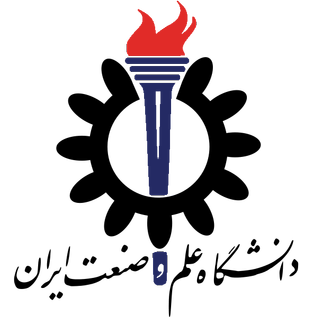
\includegraphics[width=0.5\linewidth]{images/iust.png}
    \\
    تمرین سوم Carla درس یادگیری ماشین
    }
    \author{محمد صادق پولائی موزیرجی - 403723196}
    \date{بهار 1404}

    \definecolor{dkgreen}{rgb}{0,0.6,0}
\definecolor{gray}{rgb}{0.5,0.5,0.5}
\definecolor{mauve}{rgb}{0.58,0,0.82}

\lstset{frame=tb,
  language=Python,
  aboveskip=3mm,
  belowskip=3mm,
  showstringspaces=false,
  columns=flexible,
  basicstyle={\small\ttfamily},
  numbers=none,
  numberstyle=\tiny\color{gray},
  keywordstyle=\color{blue},
  commentstyle=\color{dkgreen},
  stringstyle=\color{mauve},
  breaklines=true,
  breakatwhitespace=true,
  tabsize=3
}
\begin{document}

\maketitle
\tableofcontents
\listoffigures
\listoftables

\baselineskip = 0.85cm

\newpage
\begin{center}
  دانشکده مهندسی کامپیوتر \\
  دانشگاه علم و صنعت ایران \\[1ex]
  مدرس درس: دکتر عبدالله امیرخانی \\
  کمک مدرس: امیر خسرویان
  \vspace{2cm}
  \hrule
  \vspace{0.5cm}
  \textbf{لینک پروژه در گیت‌هاب:} \url{https://github.com/MSPoulaei/carla-instance-segmentation}
  \textbf{مدل های آموزش دیده شده:} \url{https://drive.google.com/file/d/1FJlD8G93357Z-cuRHB4xnT66y-Tx1CKk/view?usp=sharing}

\end{center}
% \newpage

\hrule
\chapter{چکیده}
این گزارش به بررسی جامع عملکرد معماری YOLOv11 در زمینه قطعه‌بندی نمونه‌ای \lr{(Instance Segmentation)} در شرایط محیطی دشوار می‌پردازد. با استفاده از شبیه‌ساز دقیق CARLA، مجموعه‌داده‌ای مصنوعی شامل چهار وضعیت جوی (روز، شب، باران، مه) تولید شد. این داده‌ها شامل چهار کلاس مهم در رانندگی خودران بودند: خودرو، اتوبوس، عابرپیاده و چراغ‌ راهنمایی. سه مدل YOLOv11 با سطوح مختلف پیچیدگی \lr{(nano, medium, large)} آموزش داده شده و از دیدگاه دقت و سرعت استنباط بررسی شدند. نتایج نشان داد که مدل YOLOv11m-seg بهترین توازن بین دقت و کارایی را فراهم می‌کند. همچنین، تکنیک‌های بهینه‌سازی مدل مانند \lr{INT8 quantization} و تبدیل به TensorRT موجب بهبود محسوس زمان اجرا شدند.

\newpage

\chapter{مقدمه}
پیشرفت سیستم‌های رانندگی خودران ذاتاً به توسعه فناوری‌های ادراک قوی و قابل اعتماد گره خورده است. یکی از مؤلفه‌های حیاتی این سیستم‌ها، توانایی تشخیص و قطعه‌بندی دقیق اشیاء در محیط اطراف است. در حالی که پیشرفت‌های چشمگیری در حوزه بینایی کامپیوتر حاصل شده است، عملکرد مدل‌های یادگیری عمیق اغلب تحت شرایط نامساعد آب و هوایی مانند باران، مه و نور کم کاهش می‌یابد. این سناریوها مصنوعات بصری ایجاد کرده، کنتراست را کاهش داده و اشیاء را پنهان می‌کنند که چالش‌های ایمنی قابل توجهی را به همراه دارد.

هدف از این پروژه، ارزیابی کمی عملکرد مدل پیشرفته YOLOv11-seg برای قطعه‌بندی نمونه در چنین محیط‌های چالش‌برانگیزی است. هدف اصلی، درک این موضوع است که چگونه نسخه‌های مختلف مدل، که از نظر اندازه و پیچیدگی متفاوت هستند، هنگام قطعه‌بندی چهار کلاس شیء حیاتی (خودرو، اتوبوس، عابر پیاده و چراغ راهنمایی) عمل می‌کنند. برای فراهم آوردن یک محیط آزمایشی کنترل‌شده و تکرارپذیر، از شبیه‌ساز CARLA برای تولید یک مجموعه داده متنوع و چالش‌برانگیز استفاده شد.

این گزارش چرخه کامل پروژه را تشریح می‌کند، که با روش‌شناسی تولید مجموعه داده و تحلیل کامل ویژگی‌های آماری آن آغاز می‌شود. سپس مراحل پیش‌پردازش مورد نیاز برای تبدیل داده‌های خام شبیه‌سازی به فرمت مناسب برای آموزش شرح داده می‌شود. فرآیند آموزش مدل، شامل انتخاب هایپرپارامترها و نتایج، برای سه نسخه YOLOv11-seg توصیف شده است. در ادامه، یک ارزیابی جامع ارائه می‌شود که عملکرد مدل را در شرایط مختلف آب و هوایی تحلیل کرده و دقت (mAP) و سرعت استنتاج آن‌ها را مقایسه می‌کند. گزارش همچنین شامل بحثی در مورد تعادل‌های مشاهده‌شده، تأثیر کیفیت داده و مزایای تکنیک‌های بهینه‌سازی مدل است.

\chapter{تولید و تحلیل مجموعه داده}
اساس این پروژه، ایجاد یک مجموعه داده با کیفیت بالا و متنوع بود. این کار با استفاده از شبیه‌ساز CARLA، یک پلتفرم منبع‌باز برای تحقیقات رانندگی خودران، انجام شد. یک سناریوی ترافیکی بسیار شلوغ برای اطمینان از وجود یک محیط غنی و پیچیده برای جمع‌آوری داده‌ها ایجاد شد. یک وسیله نقلیه اصلی (ego-vehicle) به یک جفت سنسور همگام‌سازی‌شده مجهز شد: یک دوربین RGB برای ثبت صحنه بصری و یک دوربین قطعه‌بندی نمونه برای ارائه حاشیه‌نویسی‌های زمینی \lr{(ground truth)} با دقت پیکسلی. همگام‌سازی بین دو جریان دوربین در سطح فریم اعمال شد تا از نگاشت دقیق بین تصاویر و برچسب‌های مربوطه اطمینان حاصل شود.

برای ارزیابی استحکام مدل، داده‌ها تحت چهار شرایط آب و هوایی متمایز جمع‌آوری شدند: روز صاف، شب صاف، باران شدید در روز و مه غلیظ. برای هر شرایط، ۱۰۰۰ فریم گرفته شد که در مجموع یک مجموعه داده با ۴۰۰۰ تصویر را تشکیل داد. شبیه‌سازی با تعداد زیادی وسیله نقلیه و عابر پیاده که در حالت خلبان خودکار عمل می‌کردند، پر شد تا صحنه‌های ترافیکی پویا و واقع‌گرایانه ایجاد شود.

تحلیل دقیقی از مجموعه داده تولید شده انجام شد. مجموعه داده نهایی شامل ۴۰۰۰ تصویر و در مجموع ۱۹,۱۳۷ نمونه شیء حاشیه‌نویسی شده است. توزیع فریم‌ها در شرایط آب و هوایی کاملاً متعادل بود و برای هر یک از سناریوهای روز، شب، باران و مه ۱۰۰۰ نمونه وجود داشت. با این حال، تحلیل توزیع کلاس‌ها عدم تعادل قابل توجهی را نشان داد. کلاس‌های «خودرو» و «اتوبوس» با ۷,۸۴۵ و ۷,۸۶۲ نمونه (هر کدام تقریباً ۴۱٪ از کل) بسیار فراوان بودند. کلاس «عابر پیاده» با ۳,۳۹۰ نمونه (۱۷,۷٪) به طور متوسط حضور داشت. به طور حیاتی، کلاس «چراغ راهنمایی» با تنها ۴۰ نمونه (۰,۲٪) به شدت کم‌نمایش بود. این عدم تعادل به عنوان یک چالش کلیدی شناسایی شد که احتمالاً بر توانایی مدل در یادگیری و قطعه‌بندی دقیق چراغ‌های راهنمایی تأثیر می‌گذارد. با وجود عدم تعادل کلاس، حجم ۴۰۰۰ تصویری مجموعه داده به عنوان یک پایه متوسط و کافی برای یادگیری عمیق در نظر گرفته شد، با این درک واضح که افزون‌سازی داده‌ها برای آموزش قوی مدل ضروری خواهد بود.

\begin{figure}[H]
  \centering
  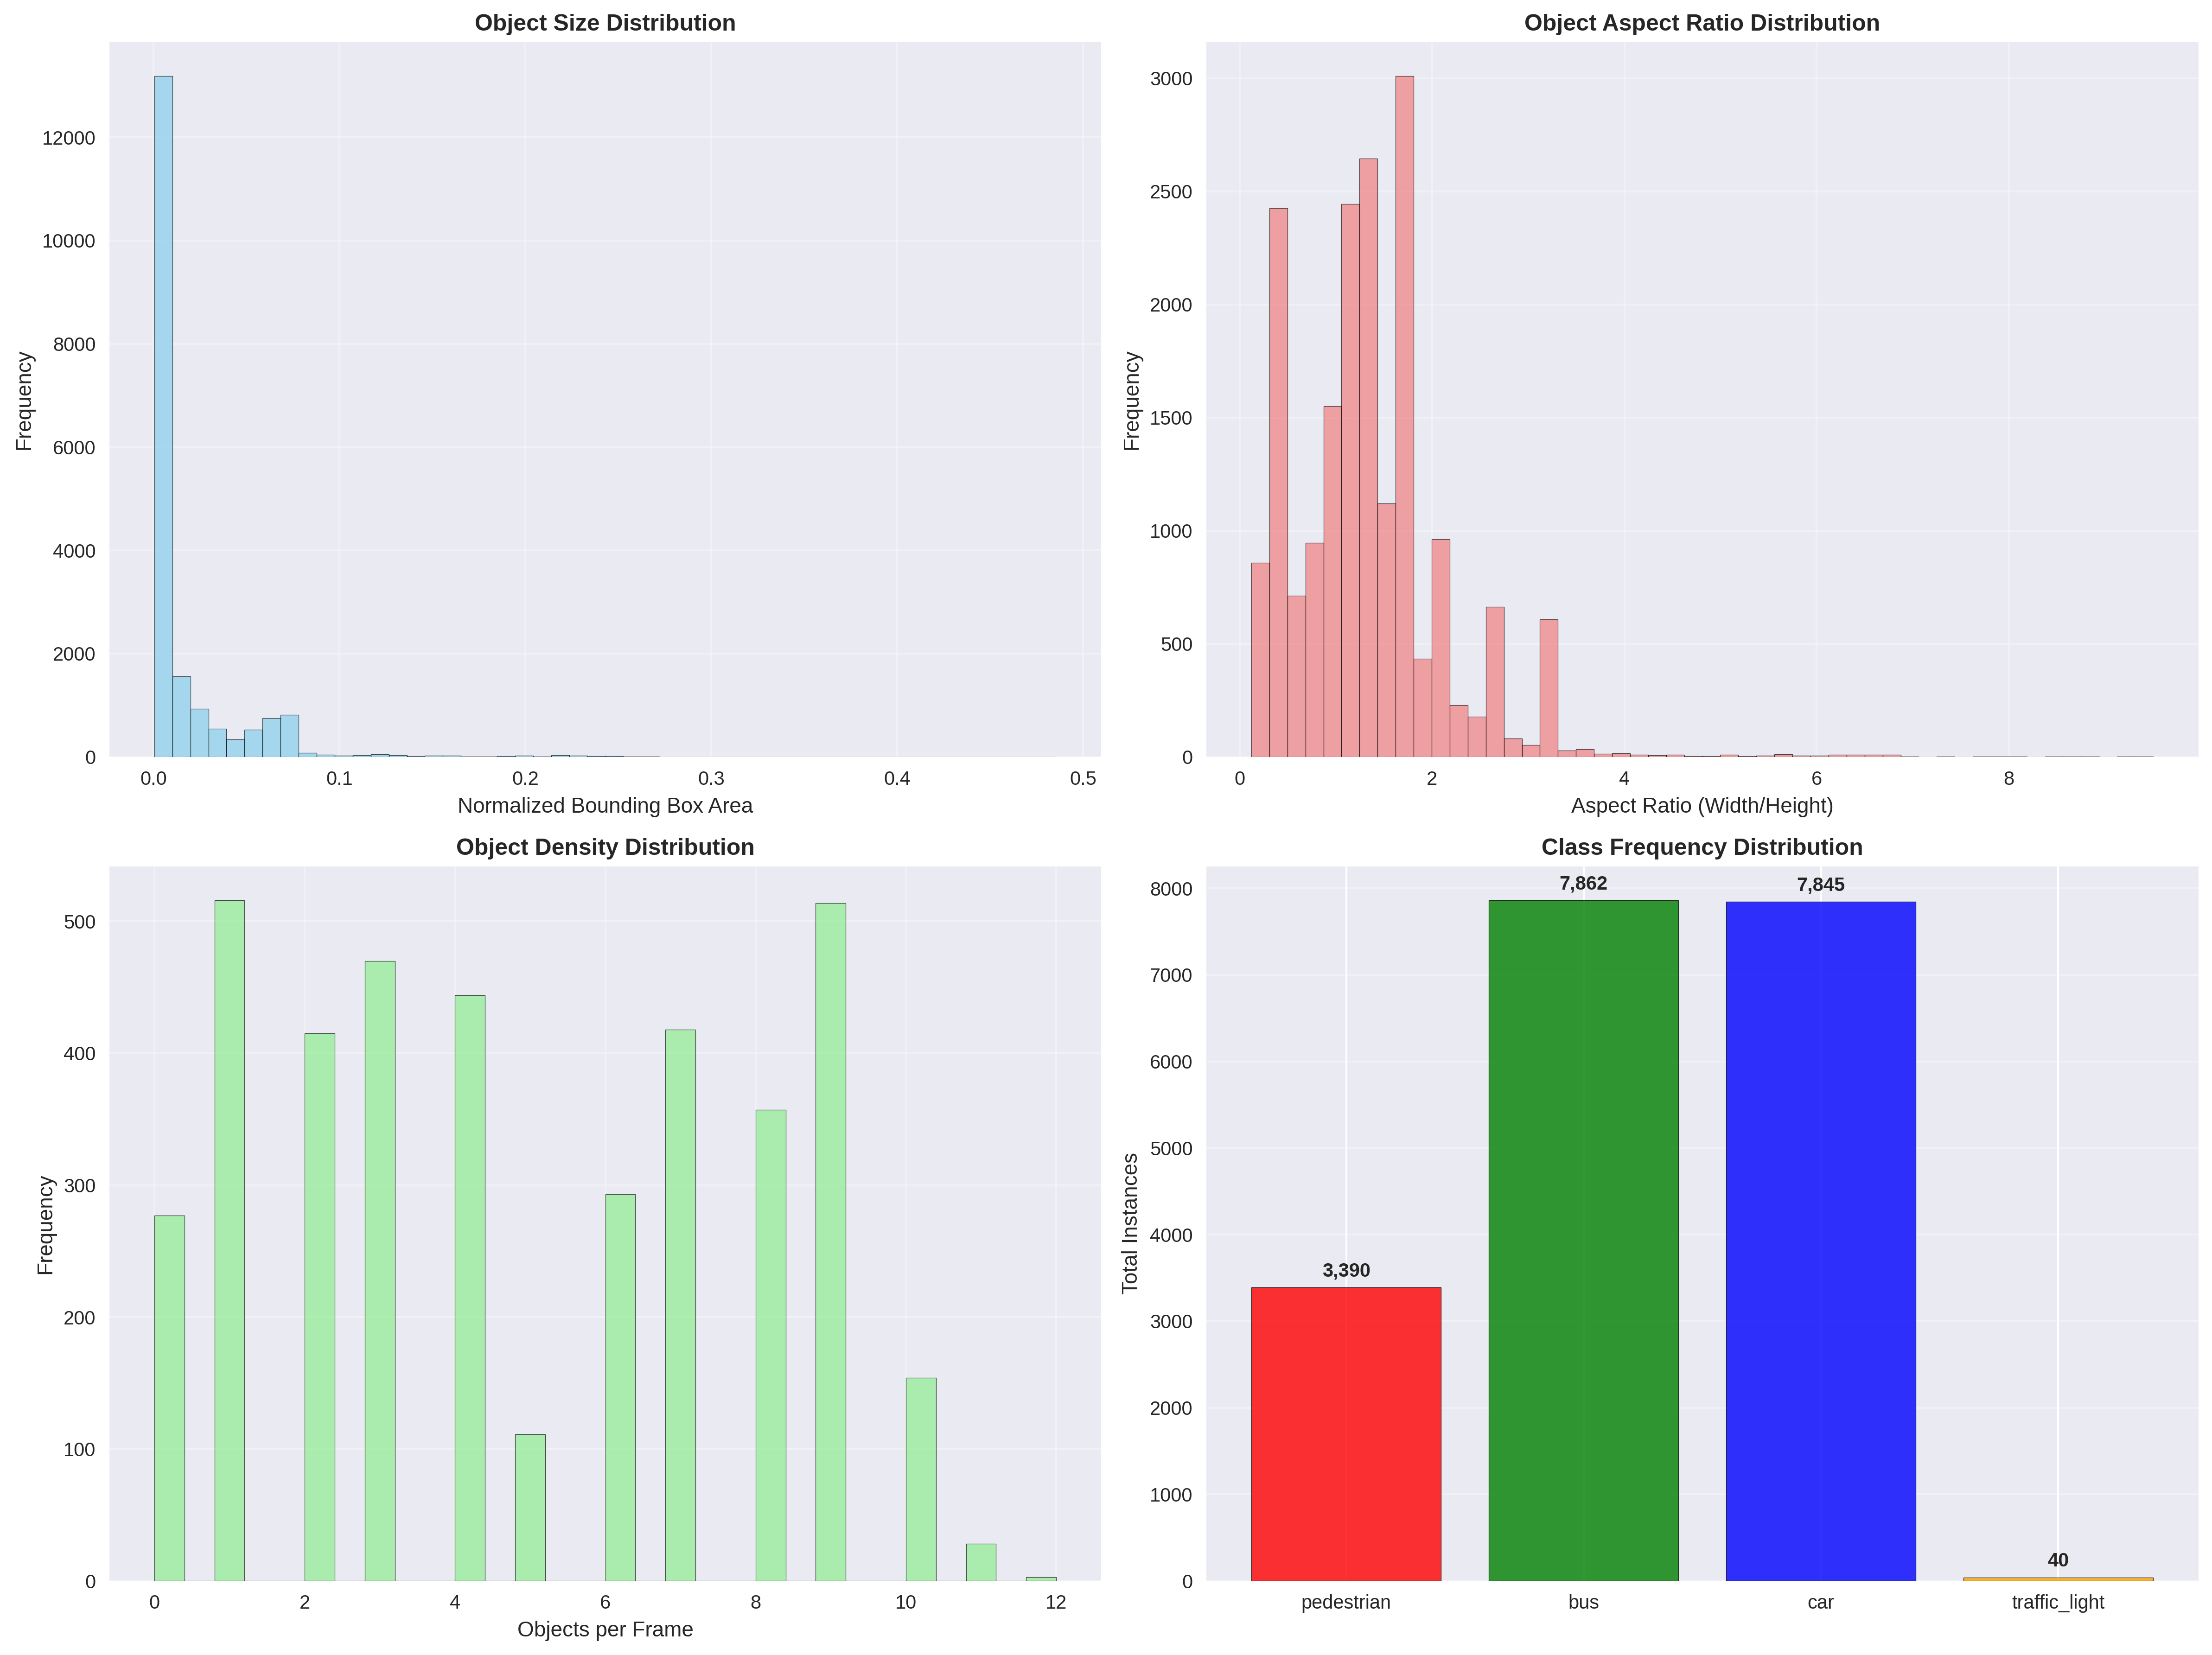
\includegraphics[width=0.8\textwidth]{images/data1/advanced_dataset_analysis.png}
  \caption{نمودارهای تحلیل مجموعه داده، شامل توزیع کلاس‌ها و شرایط آب و هوایی.}
\end{figure}

\begin{figure}[H]
  \centering
  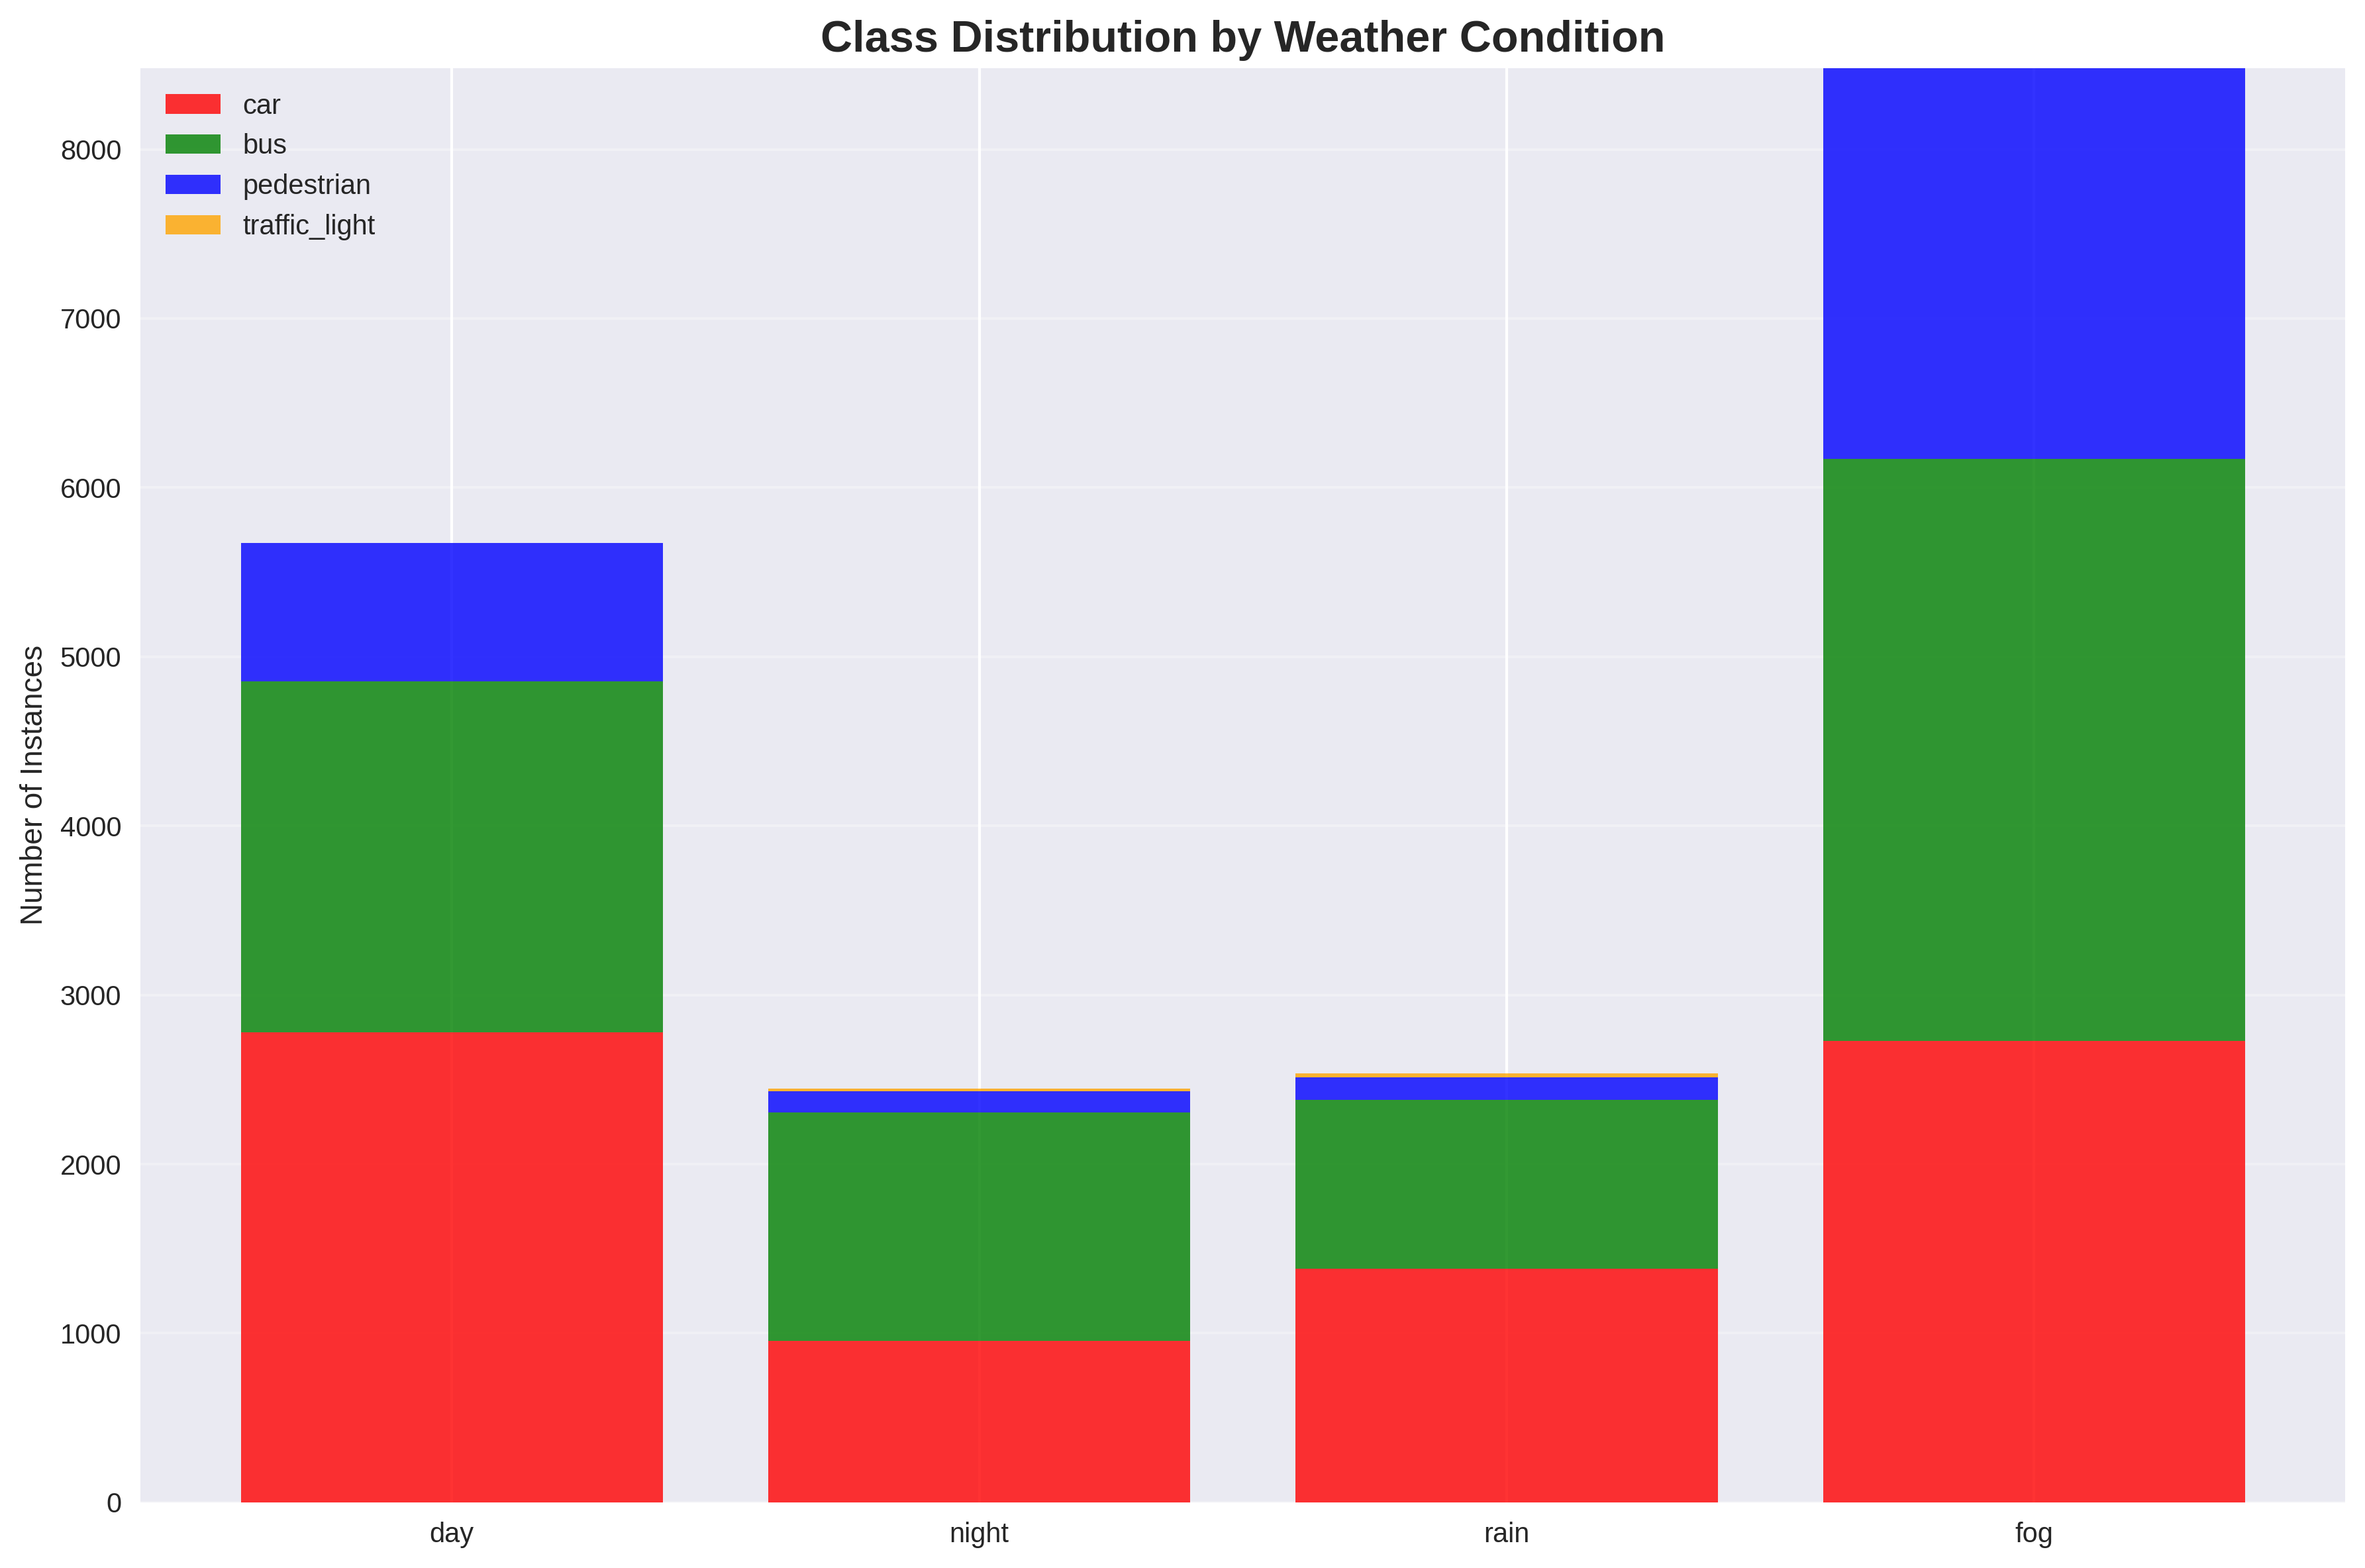
\includegraphics[width=0.8\textwidth]{images/data1/class_distribution_by_weather.png}
  \caption{نمودار توزیع کلاس‌ها بر اساس شرایط آب و هوایی}
\end{figure}

\begin{figure}[H]
  \centering
  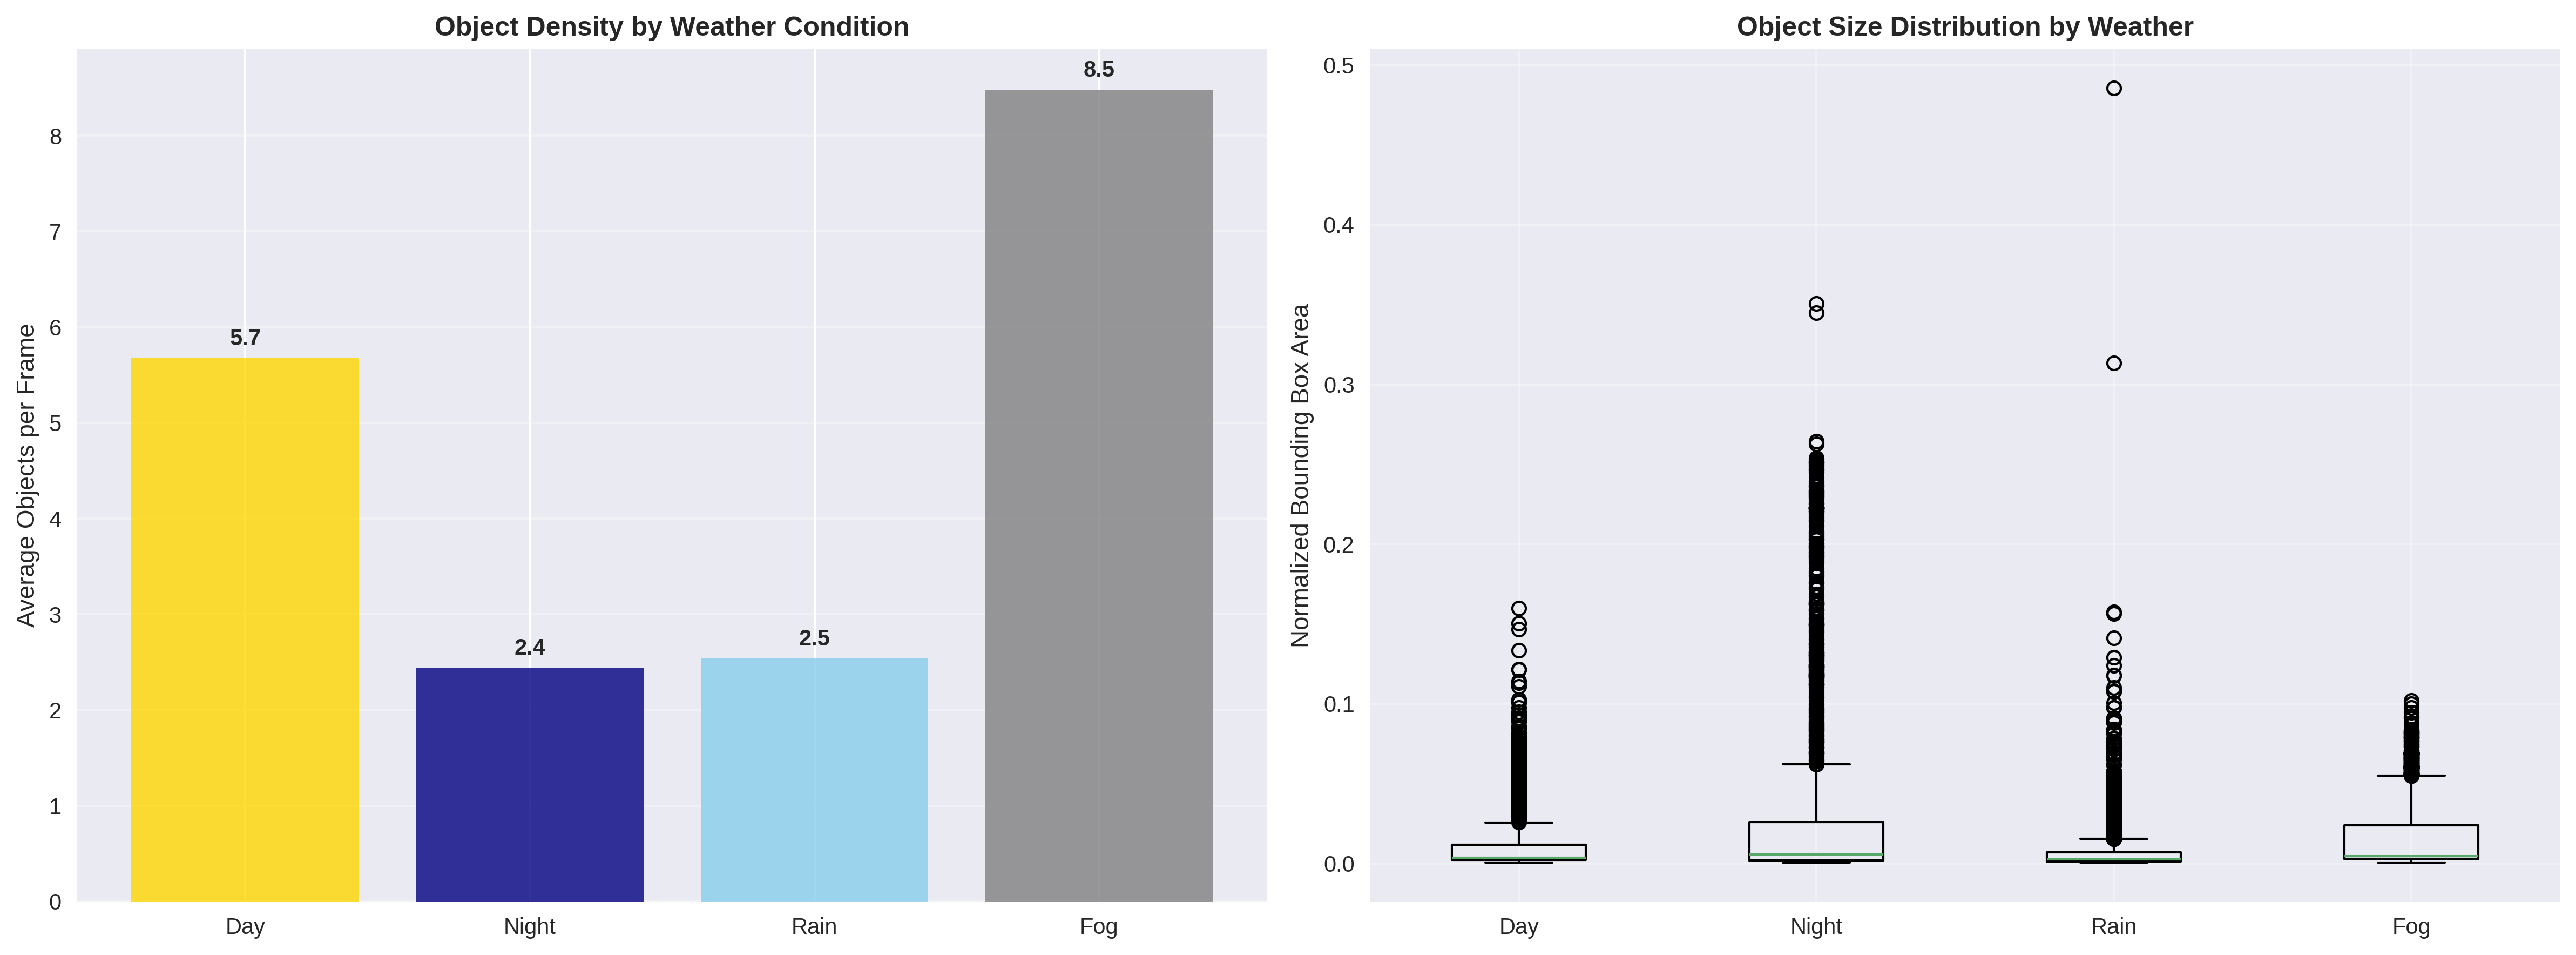
\includegraphics[width=0.8\textwidth]{images/data1/correlation_analysis.png}
  \caption{تحلیل همبستگی بین کلاس‌ها و شرایط آب و هوایی}
\end{figure}

\begin{figure}[H]
  \centering
  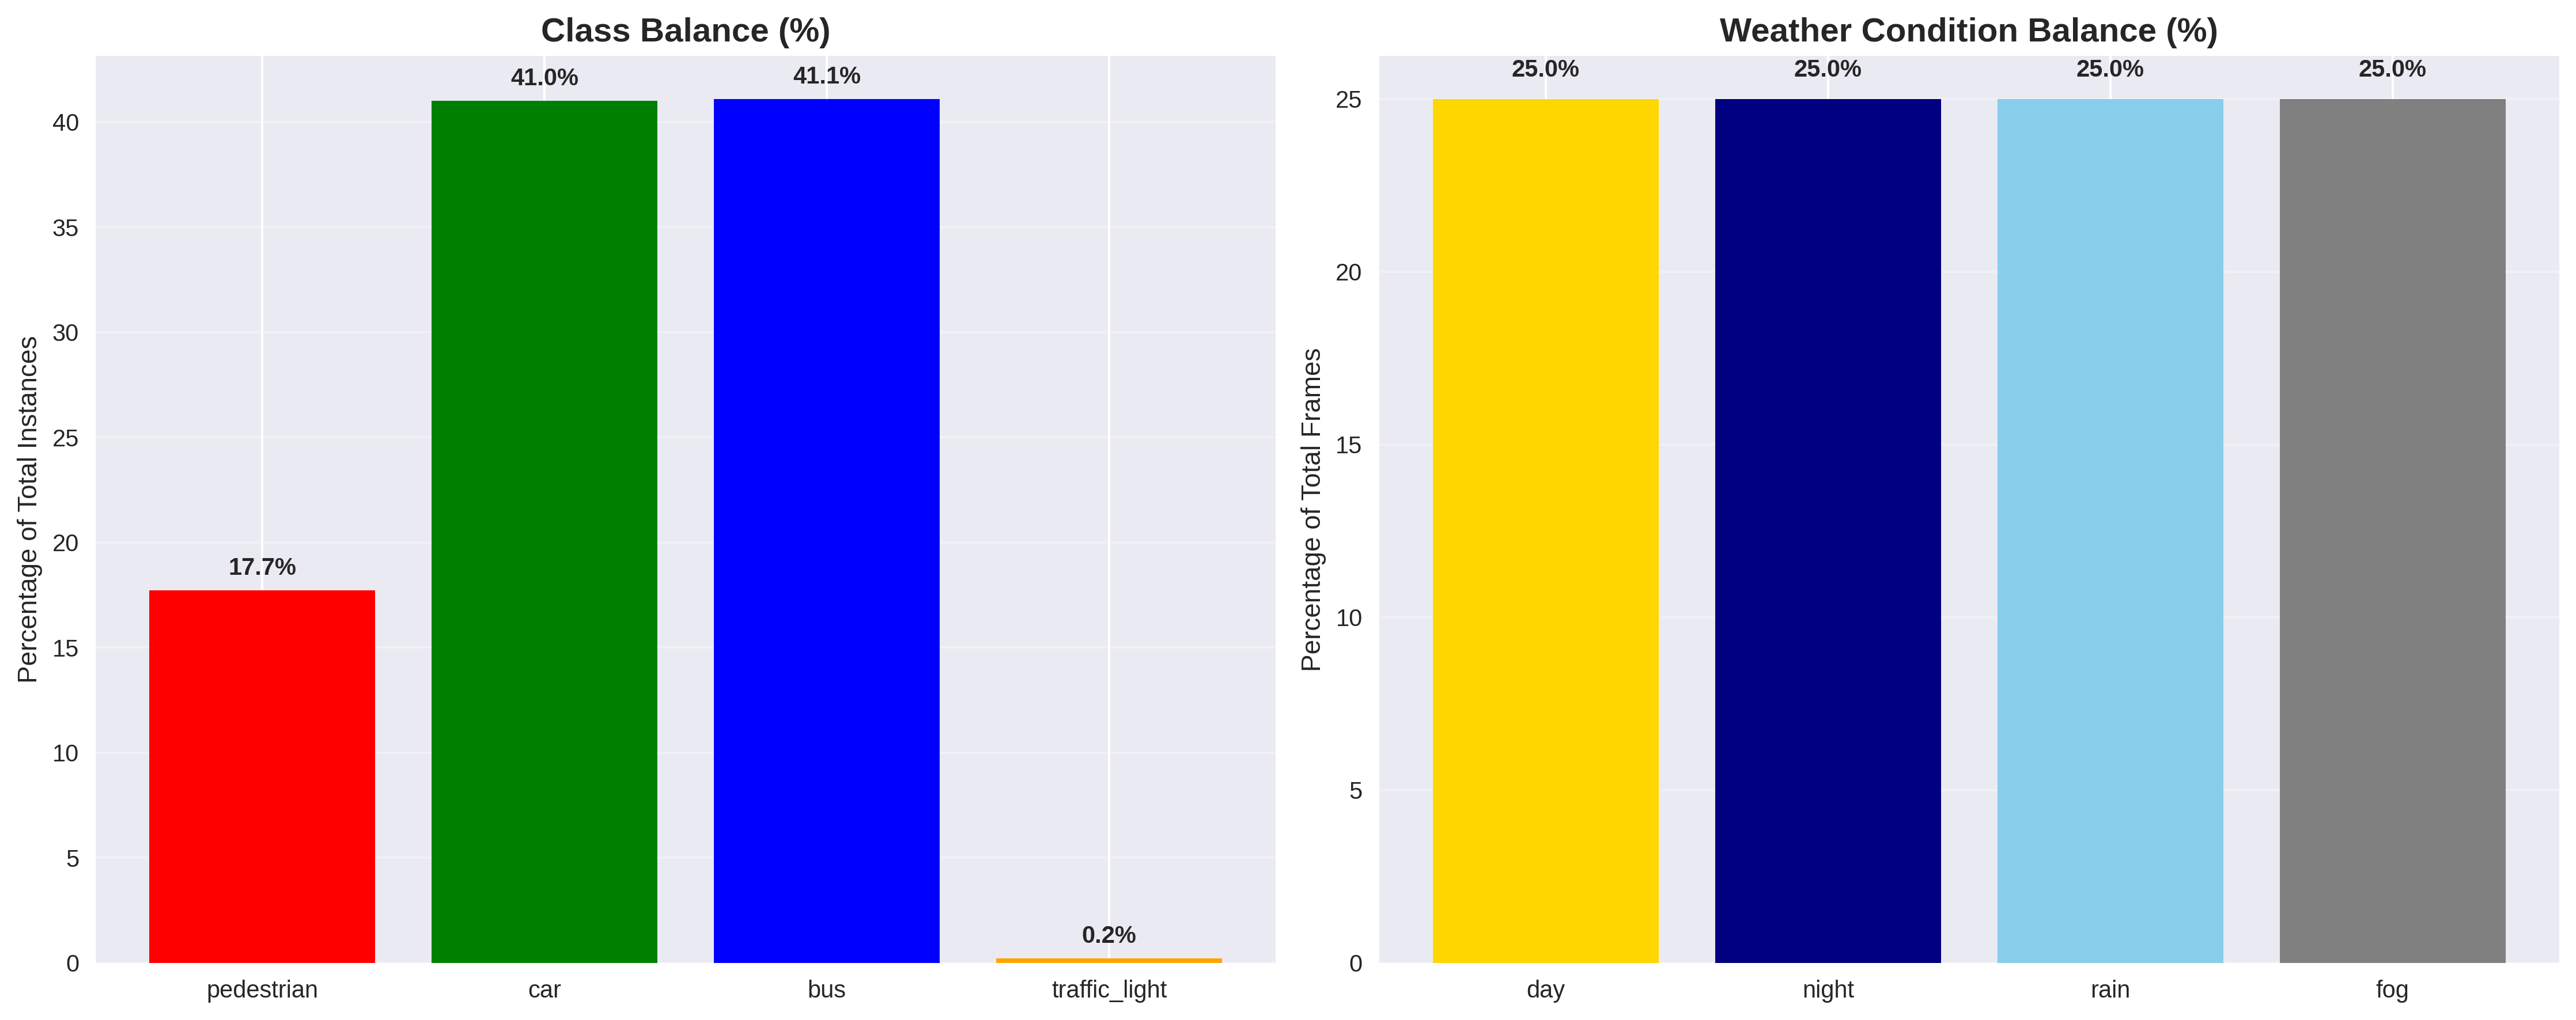
\includegraphics[width=0.8\textwidth]{images/data1/dataset_balance.png}
  \caption{نمودار توازن مجموعه داده بر اساس تعداد نمونه‌های هر کلاس}
\end{figure}

\begin{figure}[H]
  \centering
  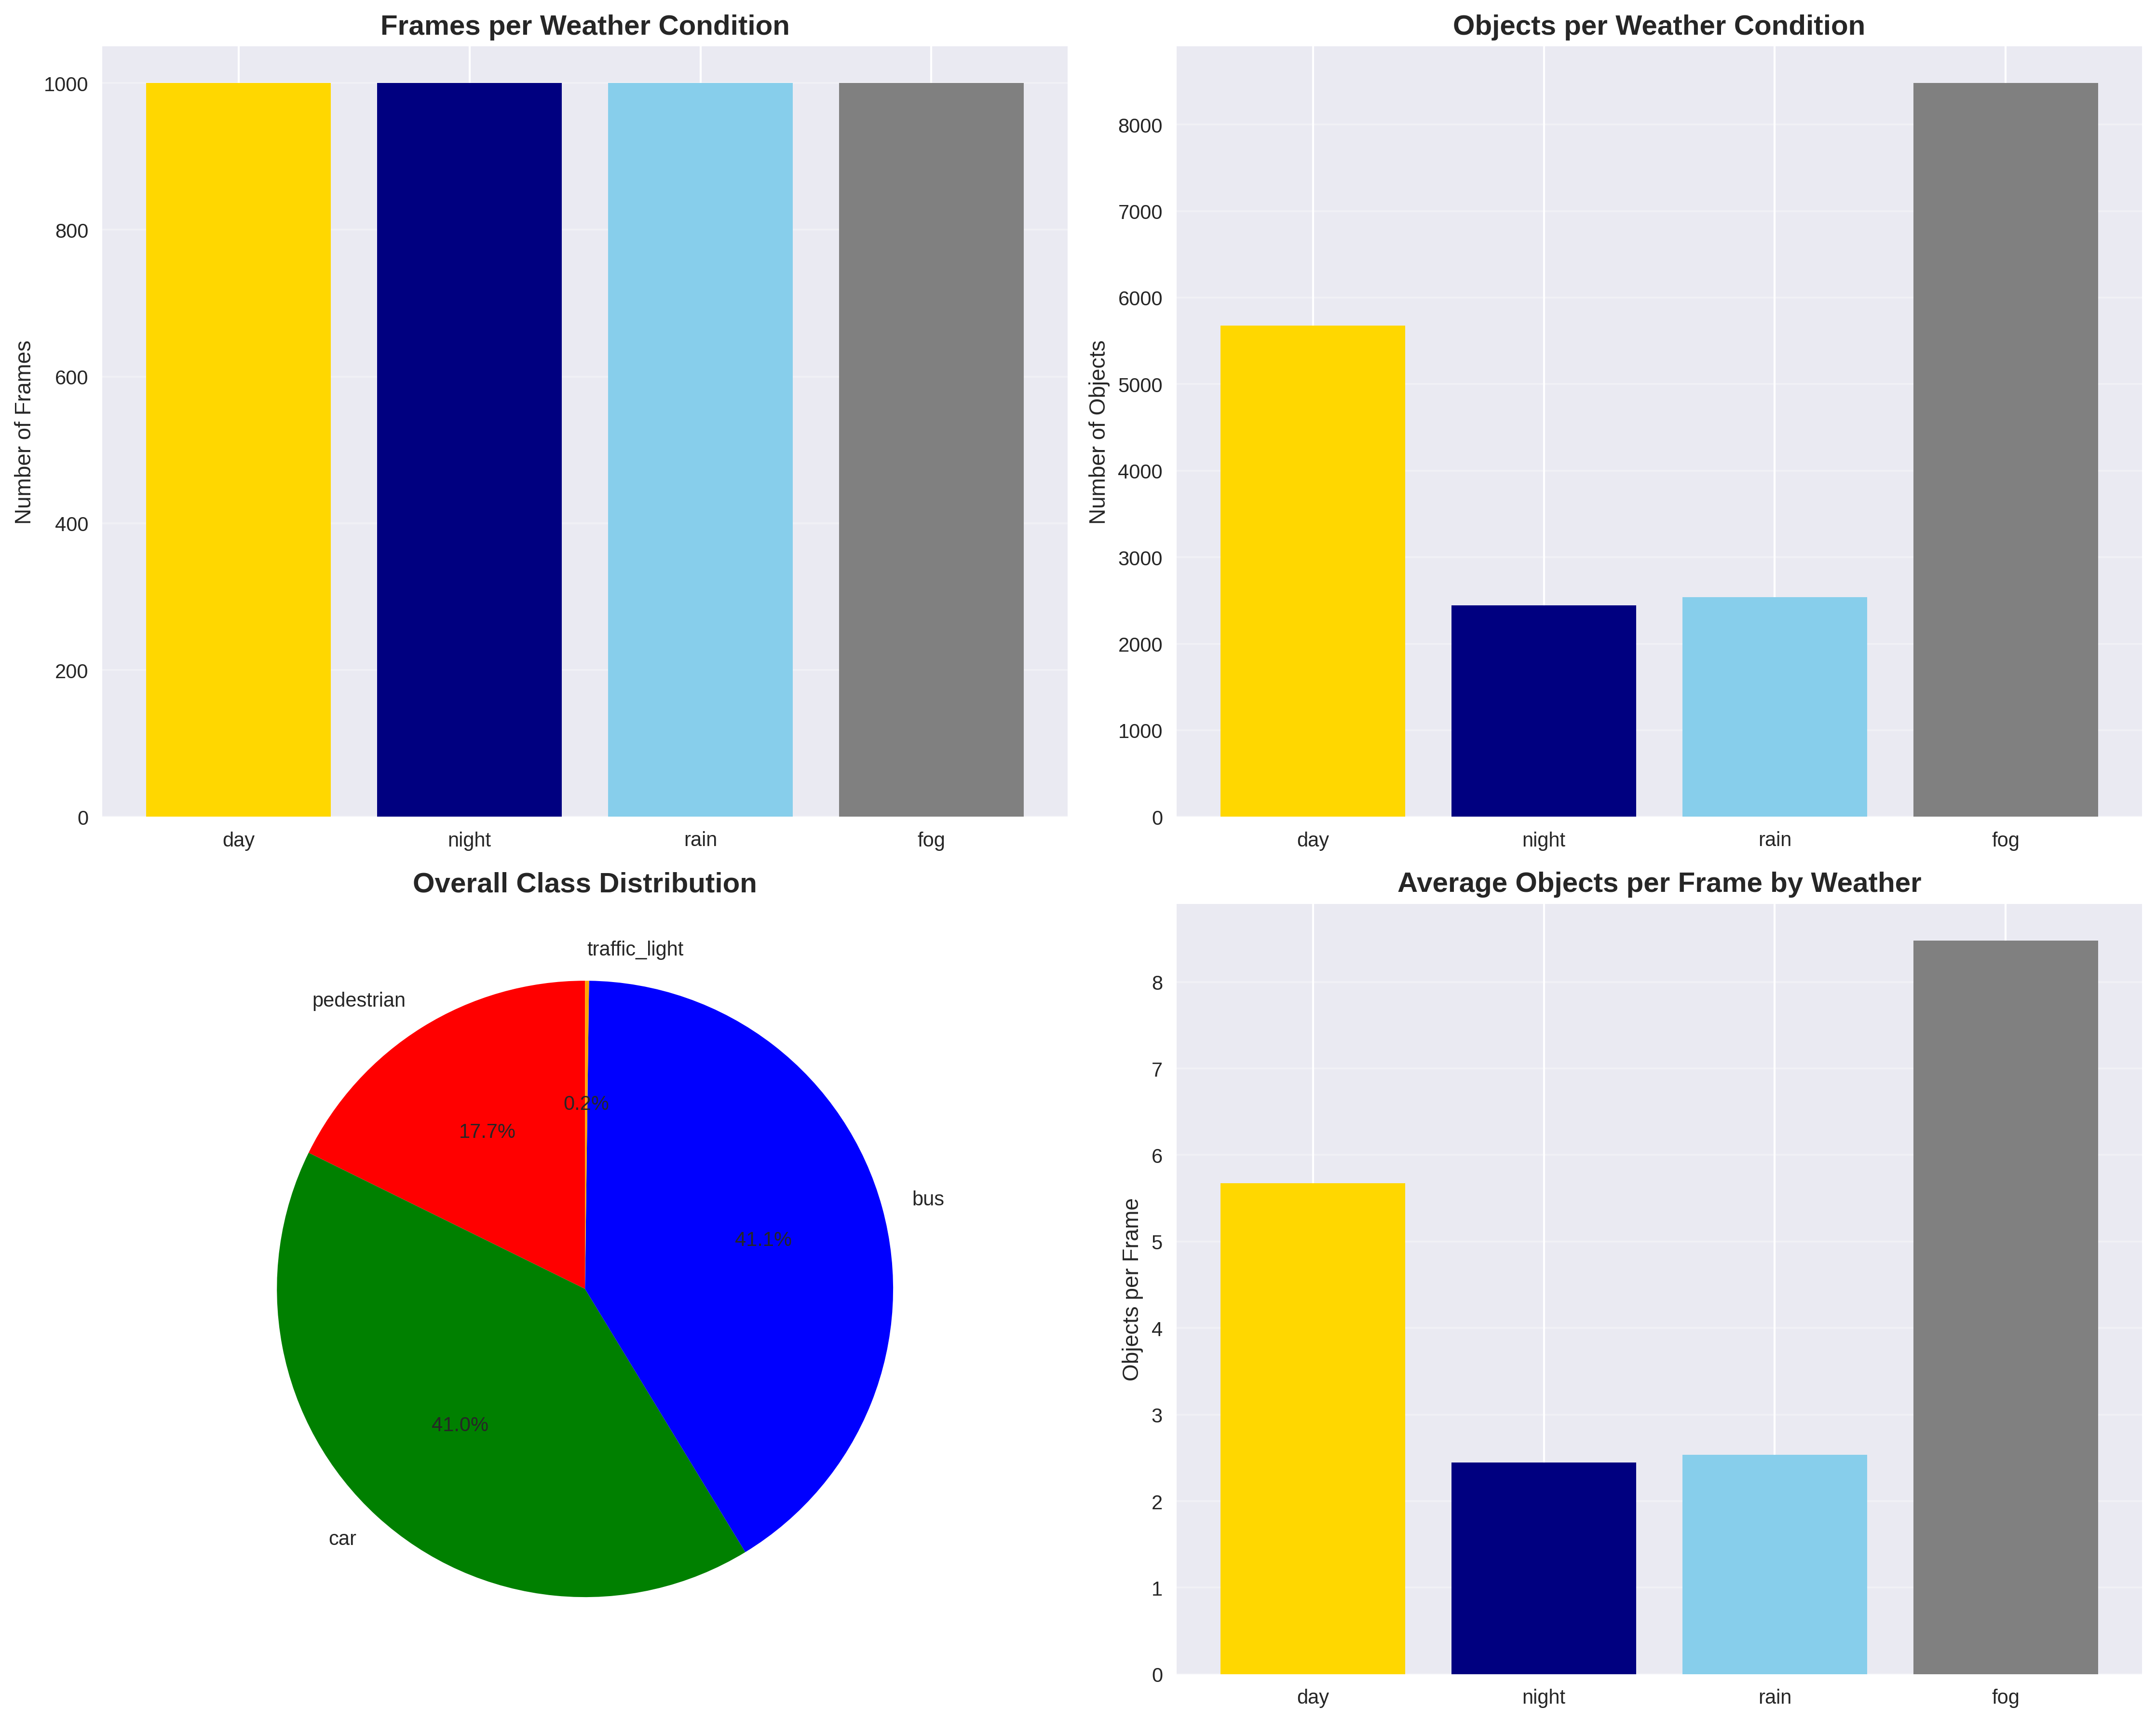
\includegraphics[width=0.8\textwidth]{images/data1/dataset_overview.png}
  \caption{نمودار نمای کلی مجموعه داده، شامل تعداد تصاویر و نمونه‌های کلی}
\end{figure}

\begin{figure}[H]
  \centering
  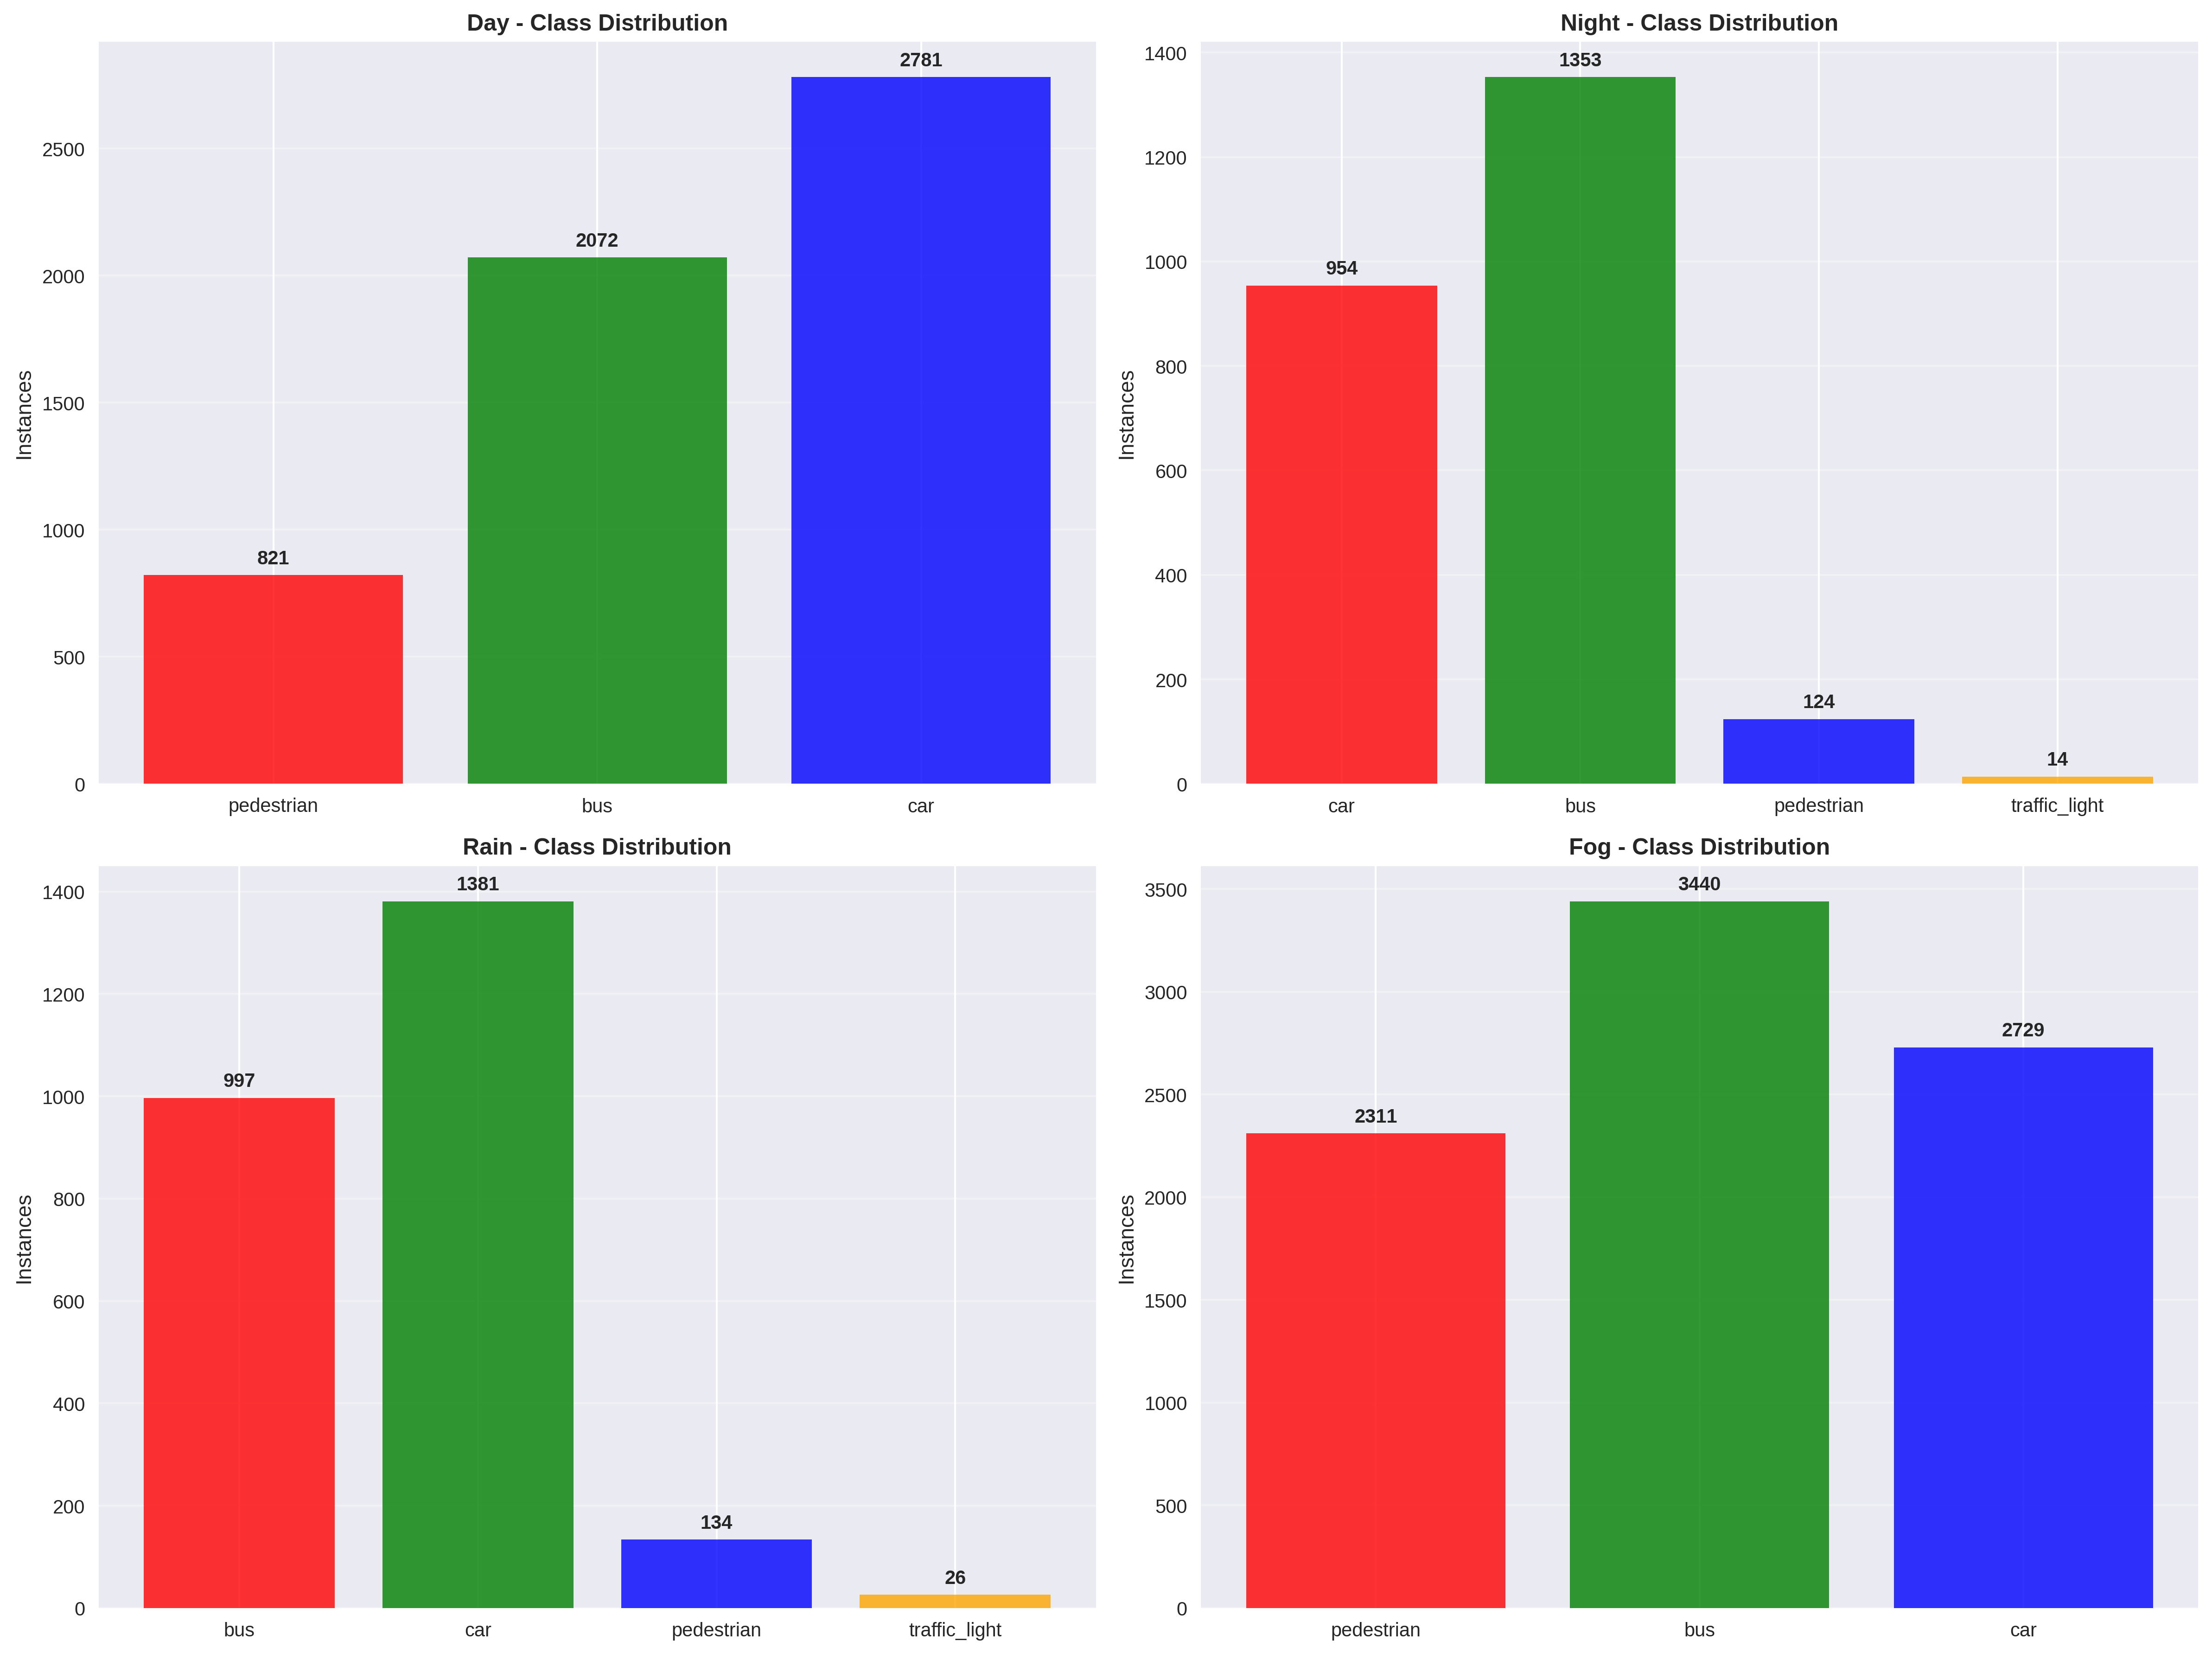
\includegraphics[width=0.8\textwidth]{images/data1/weather_specific_analysis.png}
  \caption{نمودار تحلیل خاص آب و هوا، شامل معیارهای عملکرد برای هر شرایط}
\end{figure}

\chapter{پیش‌پردازش و تقسیم‌بندی داده‌ها}
قبل از شروع آموزش مدل، داده‌های خام از CARLA نیاز به پیش‌پردازش قابل توجهی داشتند. وظیفه اصلی، تبدیل ماسک‌های قطعه‌بندی نمونه و فراداده‌های مرتبط به فرمت حاشیه‌نویسی سازگار با YOLOv11 بود. این فرمت شامل یک فایل متنی برای هر تصویر است که هر خط آن یک نمونه شیء را نشان می‌دهد. یک خط با شناسه کلاس صحیح شروع می‌شود و به دنبال آن یک سری مختصات x و y نرمال‌شده (بین ۰ تا ۱) قرار می‌گیرد که مرز چندضلعی قطعه‌بندی را مشخص می‌کند. یک اسکریپت پایتون برای خودکارسازی این تبدیل توسعه داده شد که فایل‌های JSON کارلا را تجزیه کرده، چندضلعی‌های قطعه‌بندی را برای هر شیء مورد نظر استخراج کرده و فایل‌های متنی با فرمت YOLO مربوطه را تولید می‌کرد.

پس از تبدیل تمام حاشیه‌نویسی‌ها، مجموعه داده به طور استراتژیک به مجموعه‌های آموزشی، اعتبارسنجی و آزمون تقسیم شد. نسبت تقسیم ۶۰:۲۰:۲۰ برای تخصیص اکثریت داده‌ها به آموزش و رزرو بخش‌های قابل توجهی برای اعتبارسنجی و ارزیابی عملکرد نهایی انتخاب شد. این منجر به ۲۴۰۰ تصویر برای آموزش، ۸۰۰ تصویر برای اعتبارسنجی و ۸۰۰ تصویر برای آزمون شد. برای اطمینان از ارزیابی منصفانه مدل در تمام شرایط محیطی، تقسیم‌بندی بر اساس آب و هوا لایه‌بندی شد. این امر تضمین می‌کند که هر مجموعه حاوی نسبت مساوی (۲۵٪) از تصاویر شرایط روز، شب، بارانی و مه‌آلود باشد. در نهایت، یک فایل پیکربندی `dataset.yaml` ایجاد شد. این فایل برای فریم‌ورک Ultralytics ضروری است، زیرا مسیرهای مجموعه‌های آموزشی، اعتبارسنجی و آزمون، و همچنین تعداد کلاس‌ها و نام آن‌ها را تعریف می‌کند.

\begin{figure}[H]
  \centering
  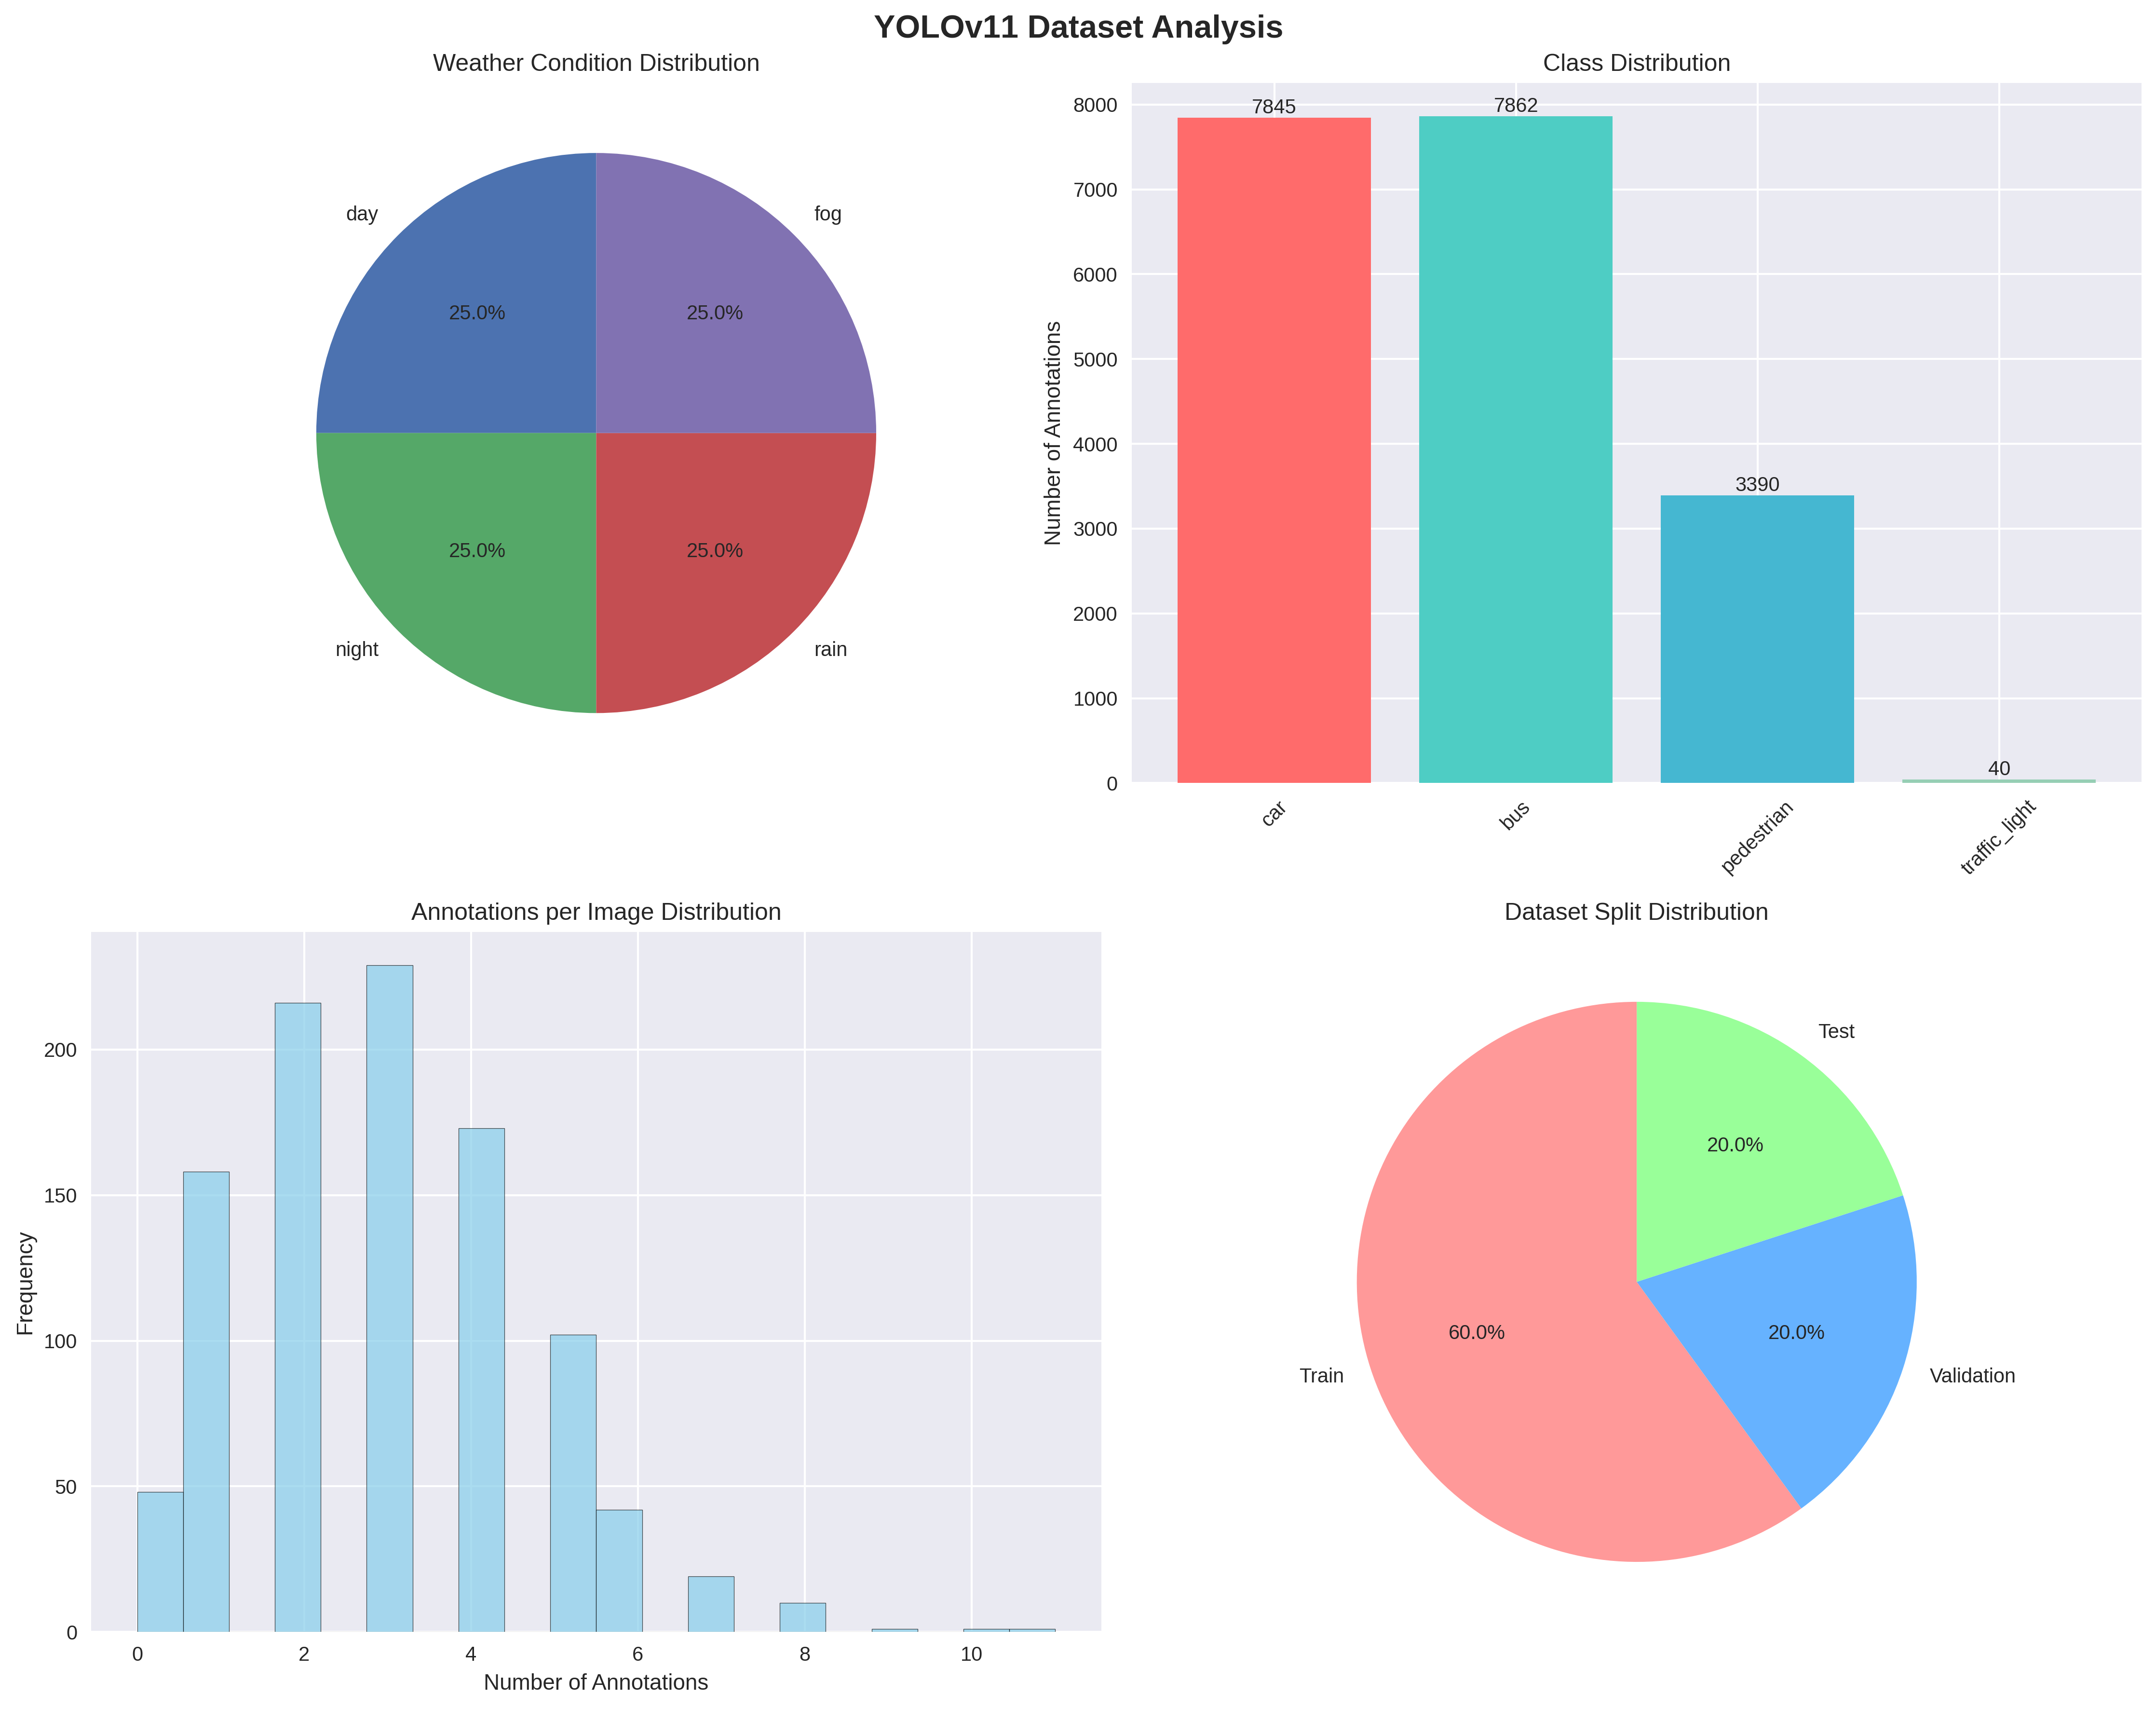
\includegraphics[width=0.8\textwidth]{images/data2/dataset_statistics.png}
  \caption{نمودار آمار مجموعه داده، شامل تعداد تصاویر و نمونه‌های کلی در مجموعه‌های آموزشی، اعتبارسنجی و آزمون}
\end{figure}
\begin{figure}[H]
  \centering
  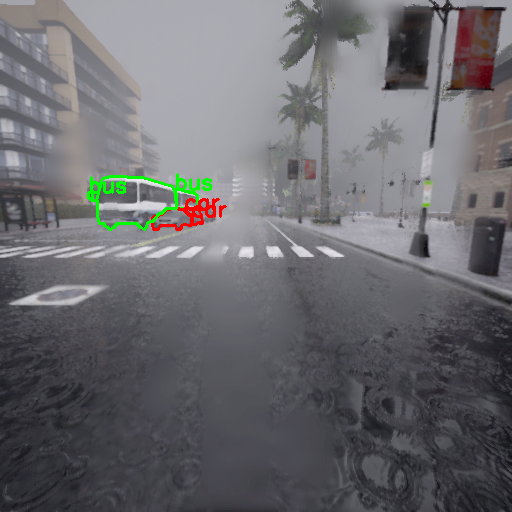
\includegraphics[width=0.8\textwidth]{images/data2/sample_10_rain_000079.png}
  \caption{نمونه‌ای از تصویر و ماسک قطعه‌بندی نمونه در شرایط بارانی}
\end{figure}
\begin{figure}[H]
  \centering
  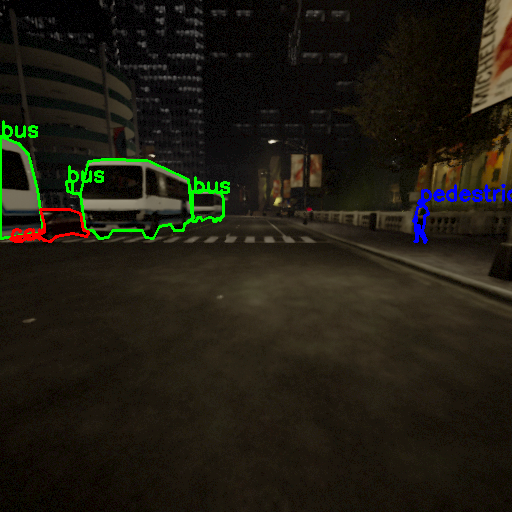
\includegraphics[width=0.8\textwidth]{images/data2/sample_8_night_000088.png}
  \caption{نمونه‌ای از تصویر و ماسک قطعه‌بندی نمونه در شرایط شب}
\end{figure}

\chapter{افزون‌سازی داده‌ها}
با توجه به اندازه متوسط مجموعه داده و عدم تعادل قابل توجه کلاس‌ها، افزون‌سازی داده‌ها یک گام حیاتی برای افزایش قابلیت تعمیم مدل و جلوگیری از بیش‌برازش (overfitting) بود. اگرچه اسکریپت نهایی آموزش از مجموعه حداقلی از افزون‌سازی‌ها برای ایجاد یک خط پایه استفاده کرد، یک خط لوله جامع افزون‌سازی با استفاده از کتابخانه Albumentations طراحی شد. این خط لوله شامل ترکیبی از تبدیلات هندسی و فتومتریک بود.

افزون‌سازی‌های هندسی مانند برگردان افقی، چرخش تصادفی و مقیاس‌بندی جزئی برای آموزش ناوردایی فضایی به مدل برنامه‌ریزی شدند. افزون‌سازی‌های فتومتریک، شامل تنظیمات روشنایی، کنتراست و اشباع، برای شبیه‌سازی تغییرات در شرایط نوری فراتر از چهار سناریوی اصلی آب و هوایی انتخاب شدند. این خط لوله برای اعمال در حین آموزش طراحی شد تا اطمینان حاصل شود که مدل در هر دوره (epoch) یک نسخه منحصربه‌فرد از یک تصویر را می‌بیند. این افزون‌سازی‌ها برای ایجاد یک مدل قوی‌تر که بتواند در مواجهه با صحنه‌های جدید که کمی با داده‌های آموزشی متفاوت هستند، به طور قابل اعتماد عمل کند، حیاتی هستند. کم‌نمایش بودن شدید کلاس «چراغ راهنمایی» به عنوان یک محدودیت ذکر شد که در کارهای آینده می‌توان با تکنیک‌های افزون‌سازی هدفمندتر مانند copy-paste، که شامل چسباندن نمونه‌های اشیاء نادر بر روی پس‌زمینه‌های مختلف است، به آن پرداخت.

\begin{figure}[H]
  \centering
  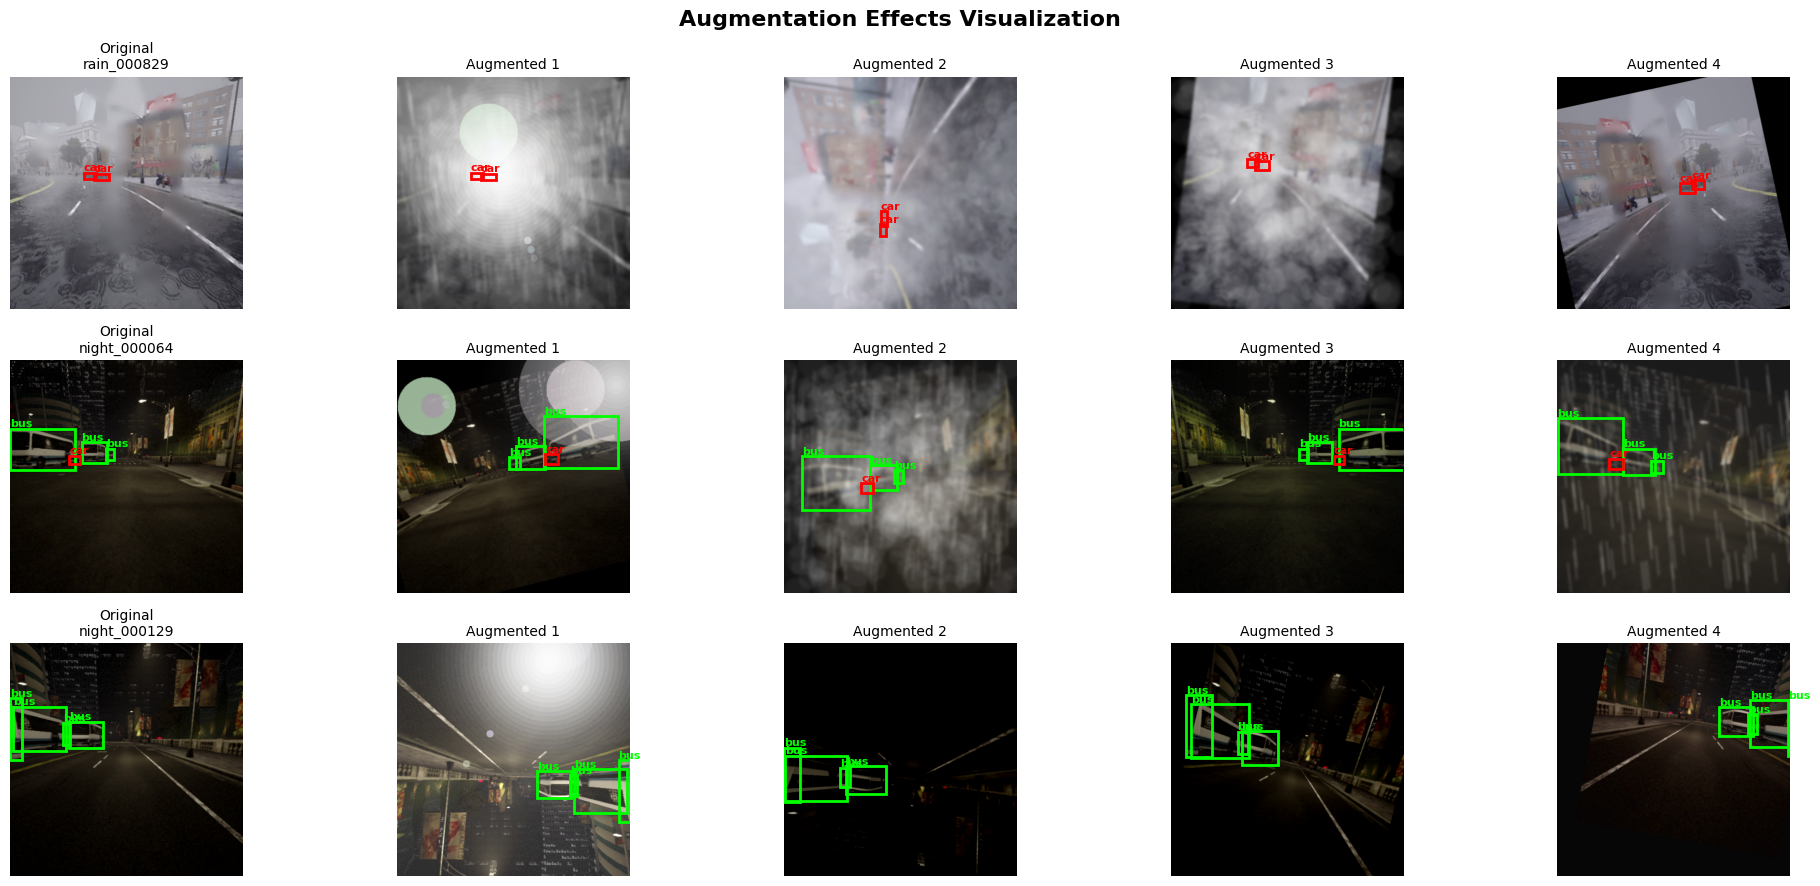
\includegraphics[width=0.8\textwidth]{images/data2/augmentation_visualization.png}
  \caption{نمونه‌هایی از تصاویر افزون‌سازی‌شده با استفاده از کتابخانه Albumentations}
\end{figure}
\begin{figure}[H]
  \centering
  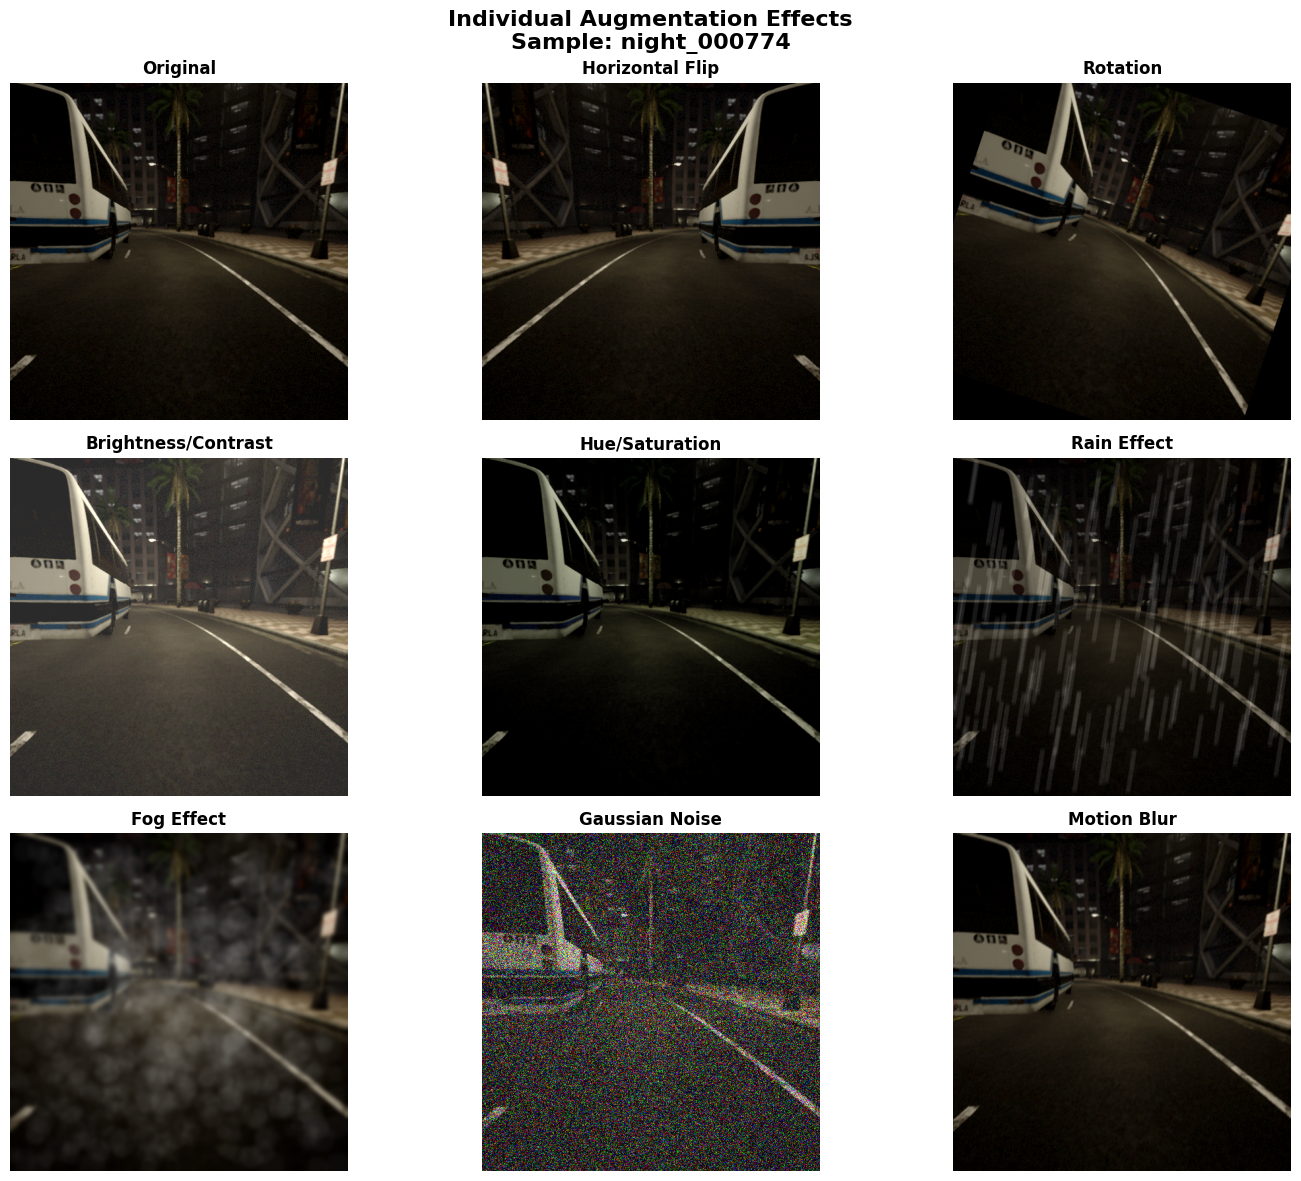
\includegraphics[width=0.8\textwidth]{images/data2/individual_augmentations.png}
  \caption{نمونه‌هایی از افزون‌سازی‌های جداگانه اعمال شده بر روی تصاویر مجموعه داده}
\end{figure}

\begin{figure}[H]
  \centering
  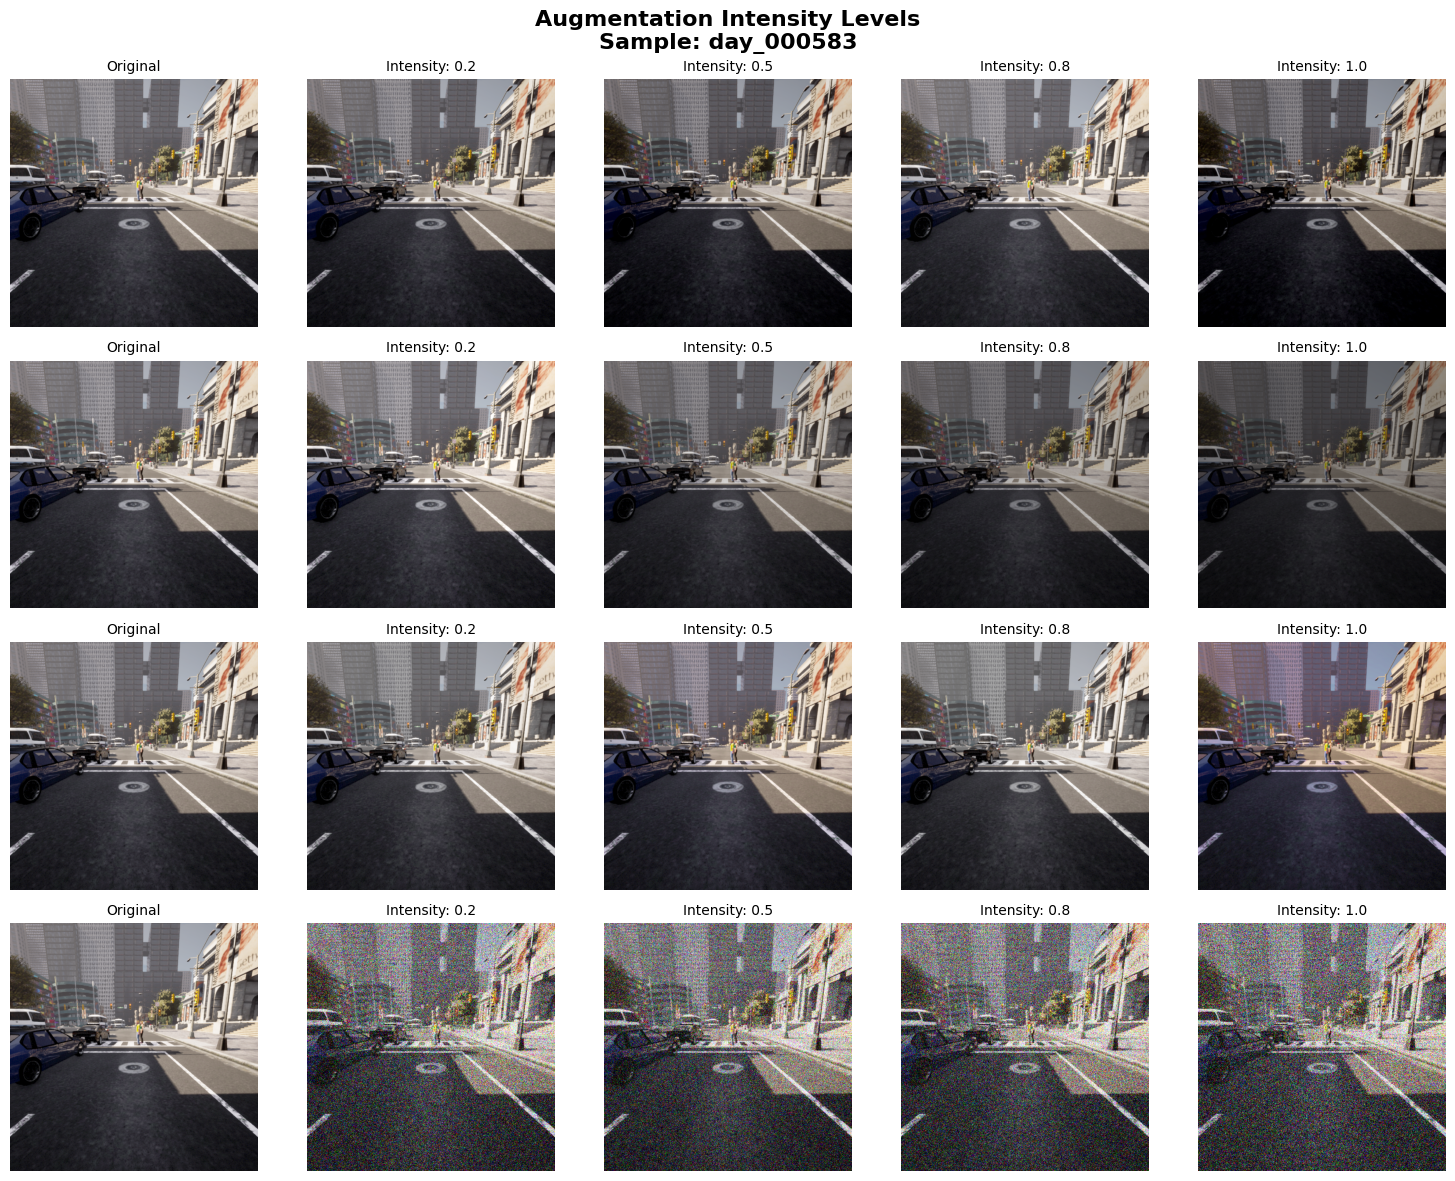
\includegraphics[width=0.8\textwidth]{images/data2/augmentation_intensity.png}
  \caption  {نمودار شدت افزون‌سازی، نشان‌دهنده توزیع شدت افزون‌سازی‌های مختلف اعمال شده}
\end{figure}

\chapter{آموزش مدل}
هسته مرحله آزمایشی شامل آموزش سه نسخه متمایز از مدل قطعه‌بندی YOLOv11 بود: YOLOv11n-seg (نانو)، YOLOv11m-seg (متوسط) و YOLOv11l-seg (بزرگ). این نسخه‌ها طیفی از پیچیدگی را ارائه می‌دهند، که مدل نانو کوچکترین و سریعترین و مدل بزرگ پیچیده‌ترین و از نظر محاسباتی سنگین‌ترین است. همه مدل‌ها از وزن‌های از پیش آموزش‌دیده بر روی مجموعه داده COCO شروع به آموزش کردند.

آموزش بر روی سیستمی مجهز به پردازنده گرافیکی \lr{NVIDIA GeForce RTX 3060} انجام شد. یک مجموعه ثابت از هایپرپارامترها در تمام سه دوره آموزش برای اطمینان از مقایسه منصفانه استفاده شد. مدل‌ها برای ۵۰ دوره با اندازه تصویر ۵۱۲x۵۱۲ و اندازه دسته ۳۲ آموزش داده شدند. بهینه‌ساز AdamW با نرخ یادگیری اولیه ۰,۰۱ انتخاب شد. برای اطمینان از پایداری آموزش، از یک مرحله گرم‌کردن (warm-up) به مدت ۳ دوره استفاده شد. فرآیند آموزش با استفاده از TensorBoard به دقت نظارت شد، که تجسم‌های بی‌درنگ از معیارهای کلیدی مانند خطای آموزش/اعتبارسنجی و میانگین دقت متوسط (mAP) را فراهم می‌کرد.

لاگ‌های آموزش و منحنی‌های خطا برای هر سه مدل همگرایی موفقیت‌آمیز را بدون علائم قابل توجهی از بیش‌برازش نشان دادند. همانطور که انتظار می‌رفت، زمان آموزش با اندازه مدل به طور قابل توجهی متفاوت بود. مدل YOLOv11n-seg آموزش را سریع‌تر از همه به پایان رساند، در حالی که YOLOv11l-seg به طولانی‌ترین زمان نیاز داشت. وزن‌های نهایی آموزش‌دیده از دوره‌ای که بهترین mAP اعتبارسنجی را داشت برای هر نسخه مدل برای مرحله ارزیابی بعدی ذخیره شد.

\begin{figure}[H]
  \centering
  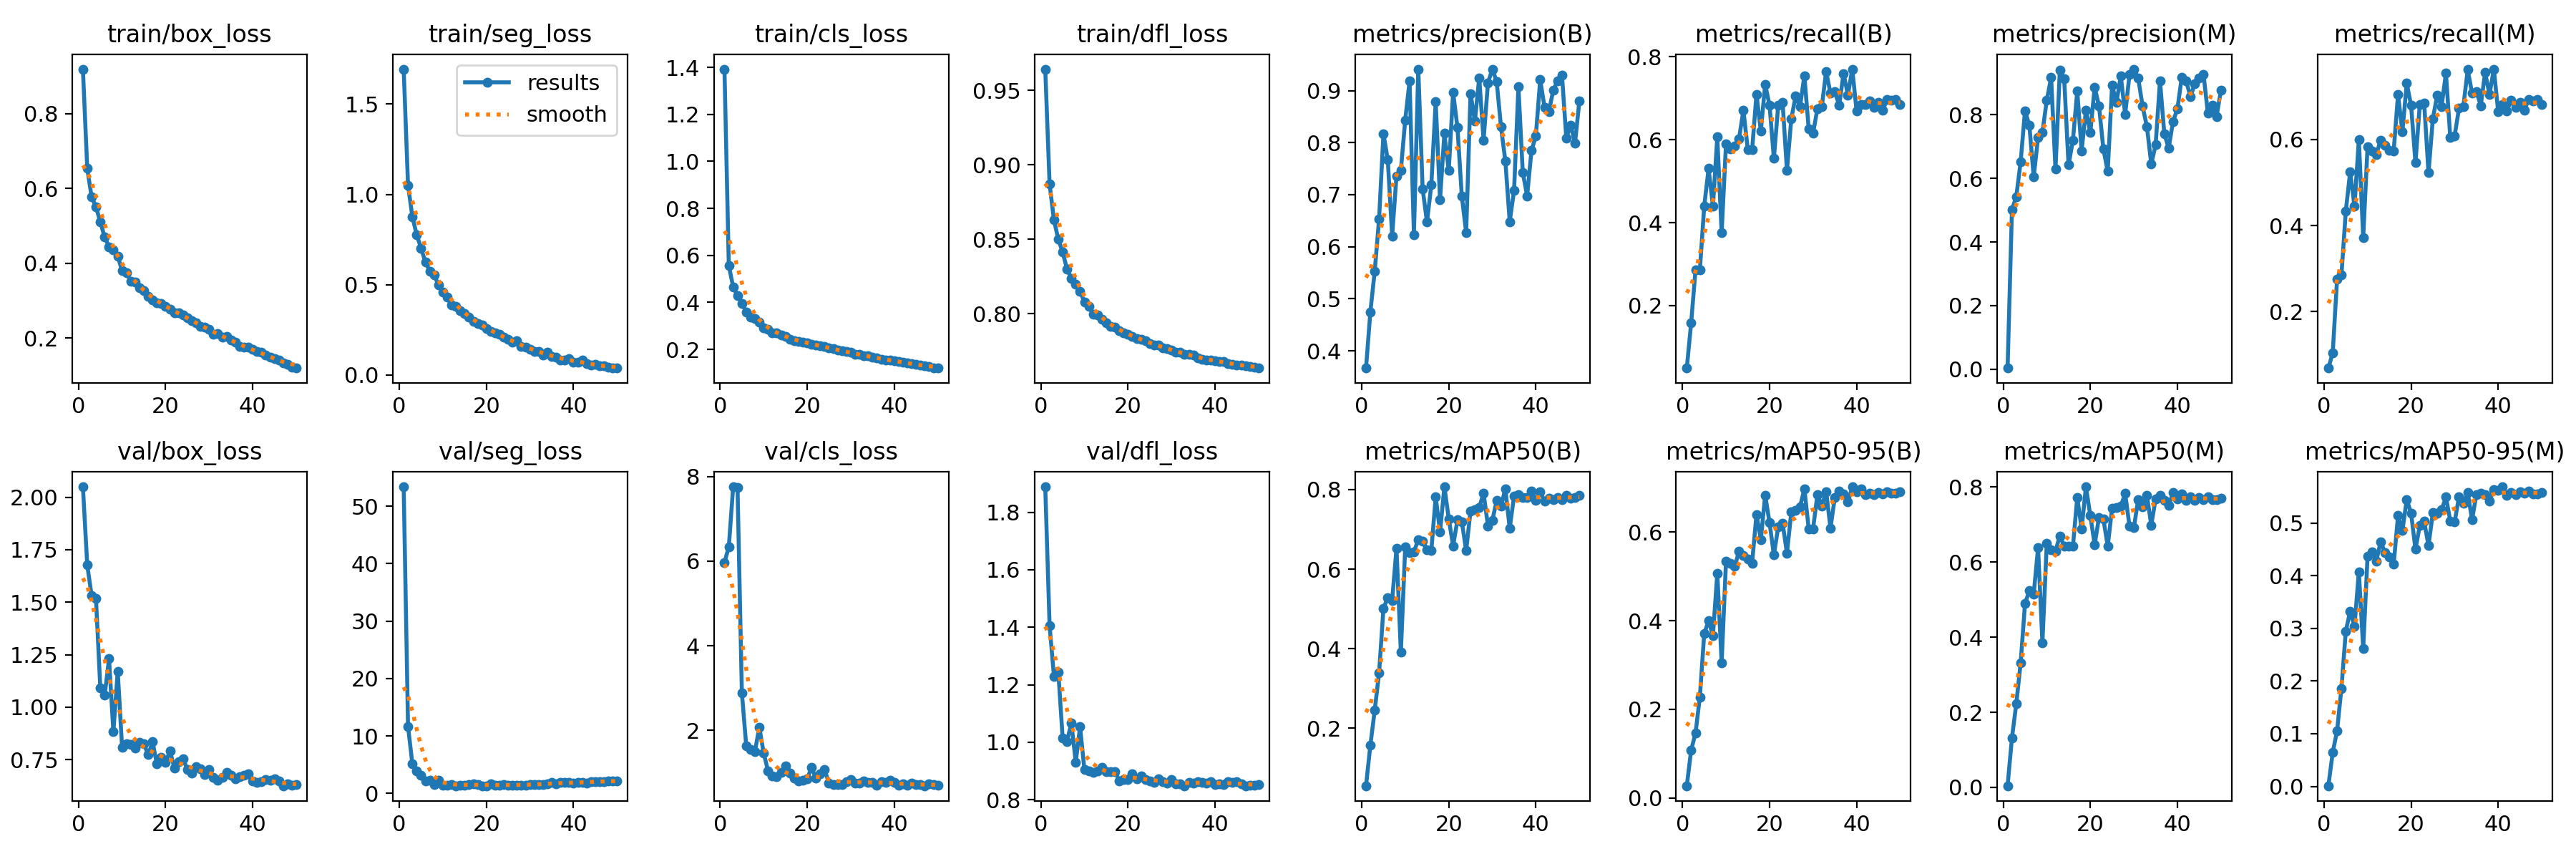
\includegraphics[width=0.8\textwidth]{images/nano/results.png}
  \caption{نمودارهای خطای آموزش و اعتبارسنجی برای مدل‌ نانو}
\end{figure}
\begin{figure}[H]
  \centering
  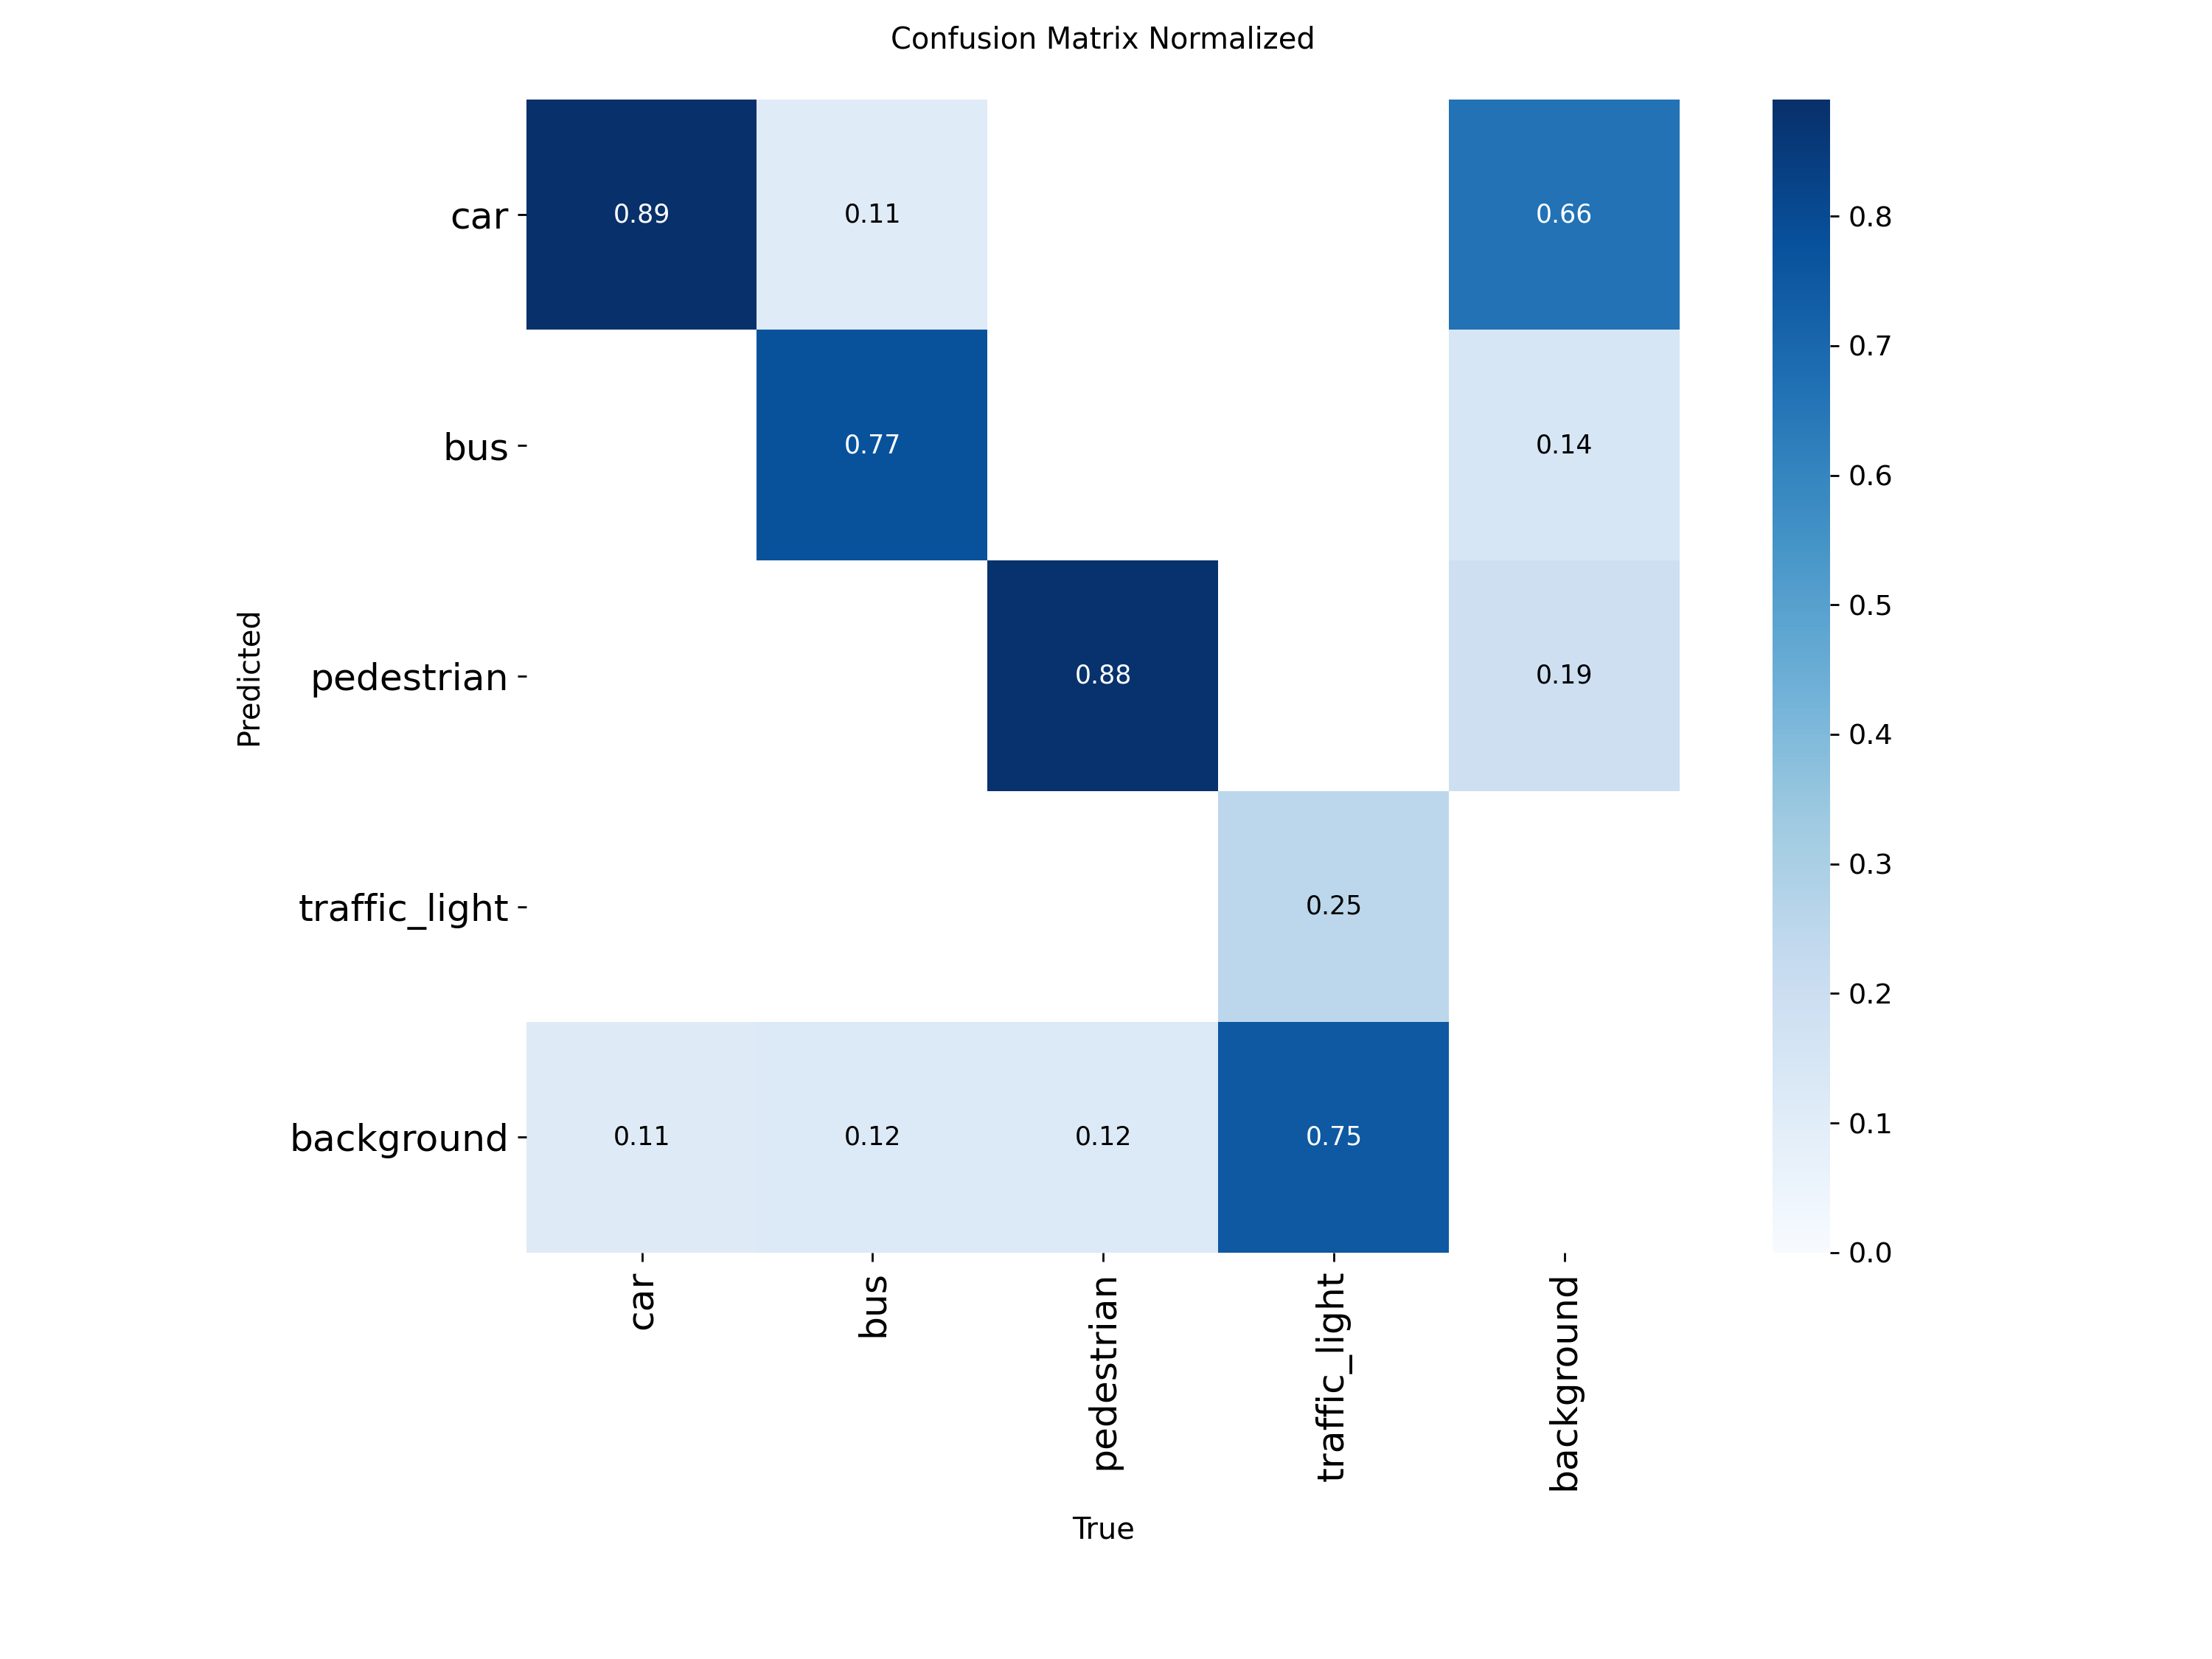
\includegraphics[width=0.8\textwidth]{images/nano/confusion_matrix_normalized.png}
  \caption{ماتریس درهم رفتگی با داده های val برای مدل نانو}
\end{figure}
\begin{figure}[H]
  \centering
  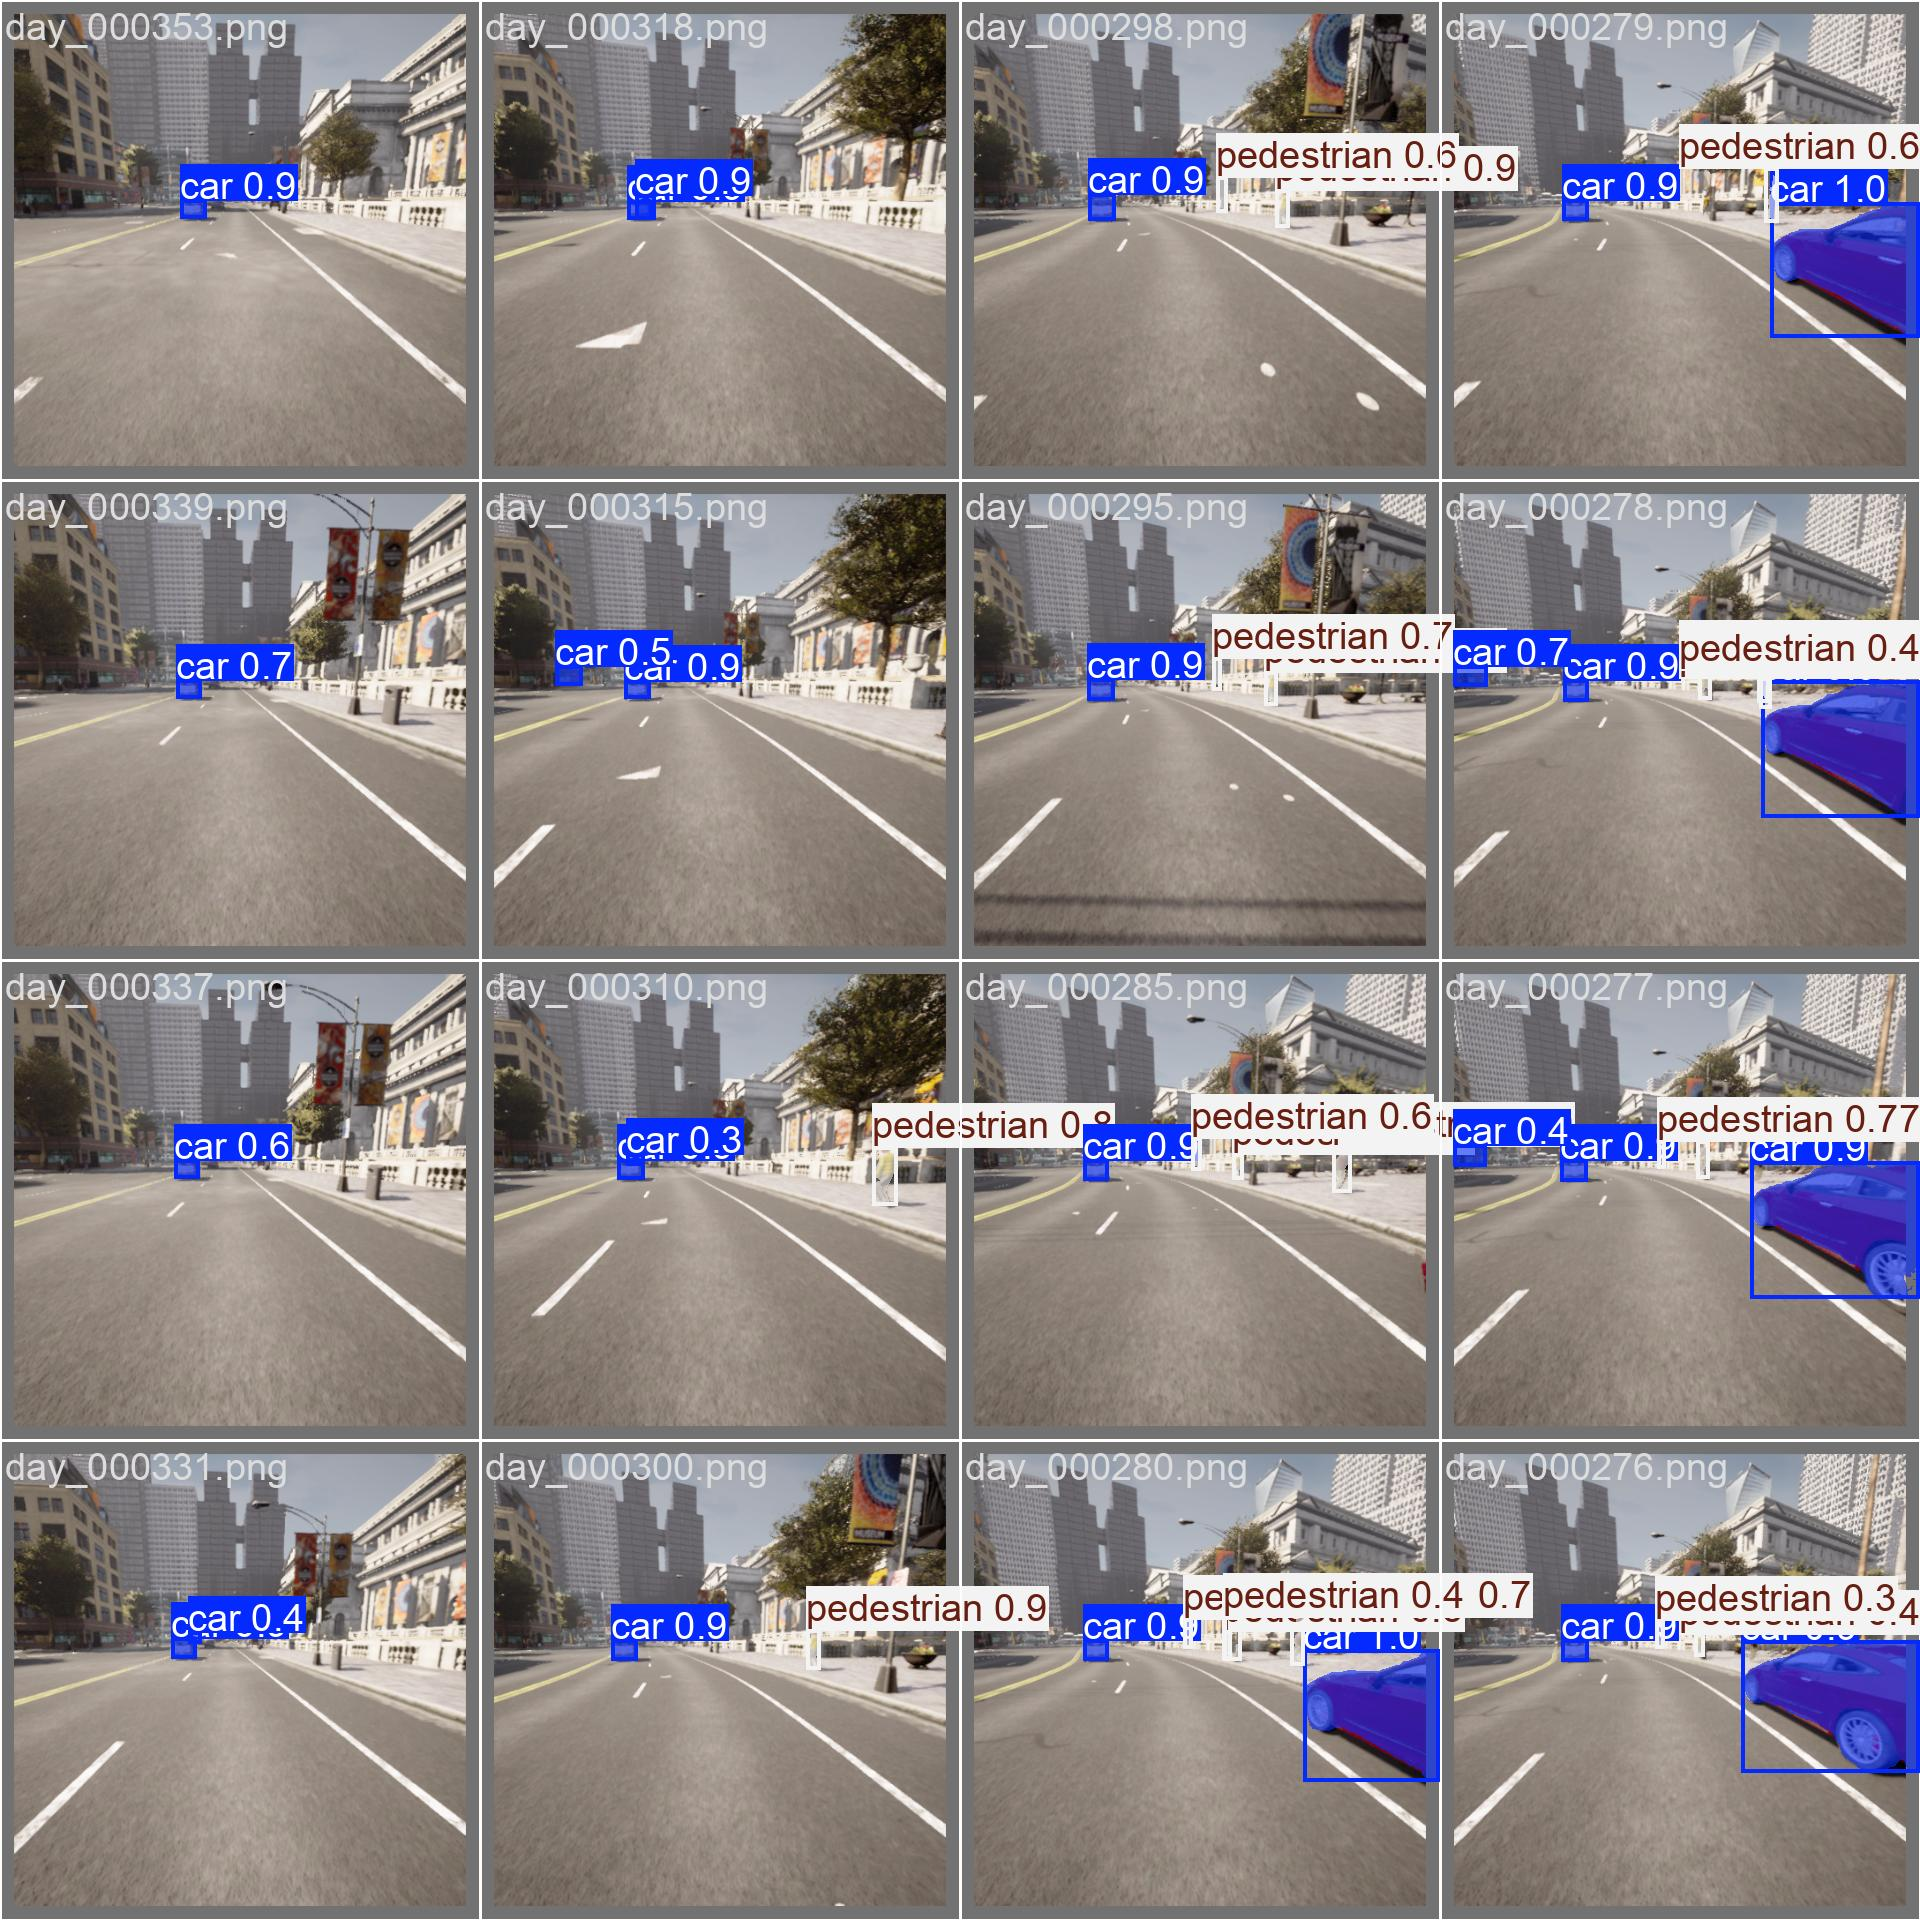
\includegraphics[width=0.8\textwidth]{images/nano/val_batch2_pred.jpg}
  \caption{تست مدل نانو بر روی داده های val}
\end{figure}

\begin{figure}[H]
  \centering
  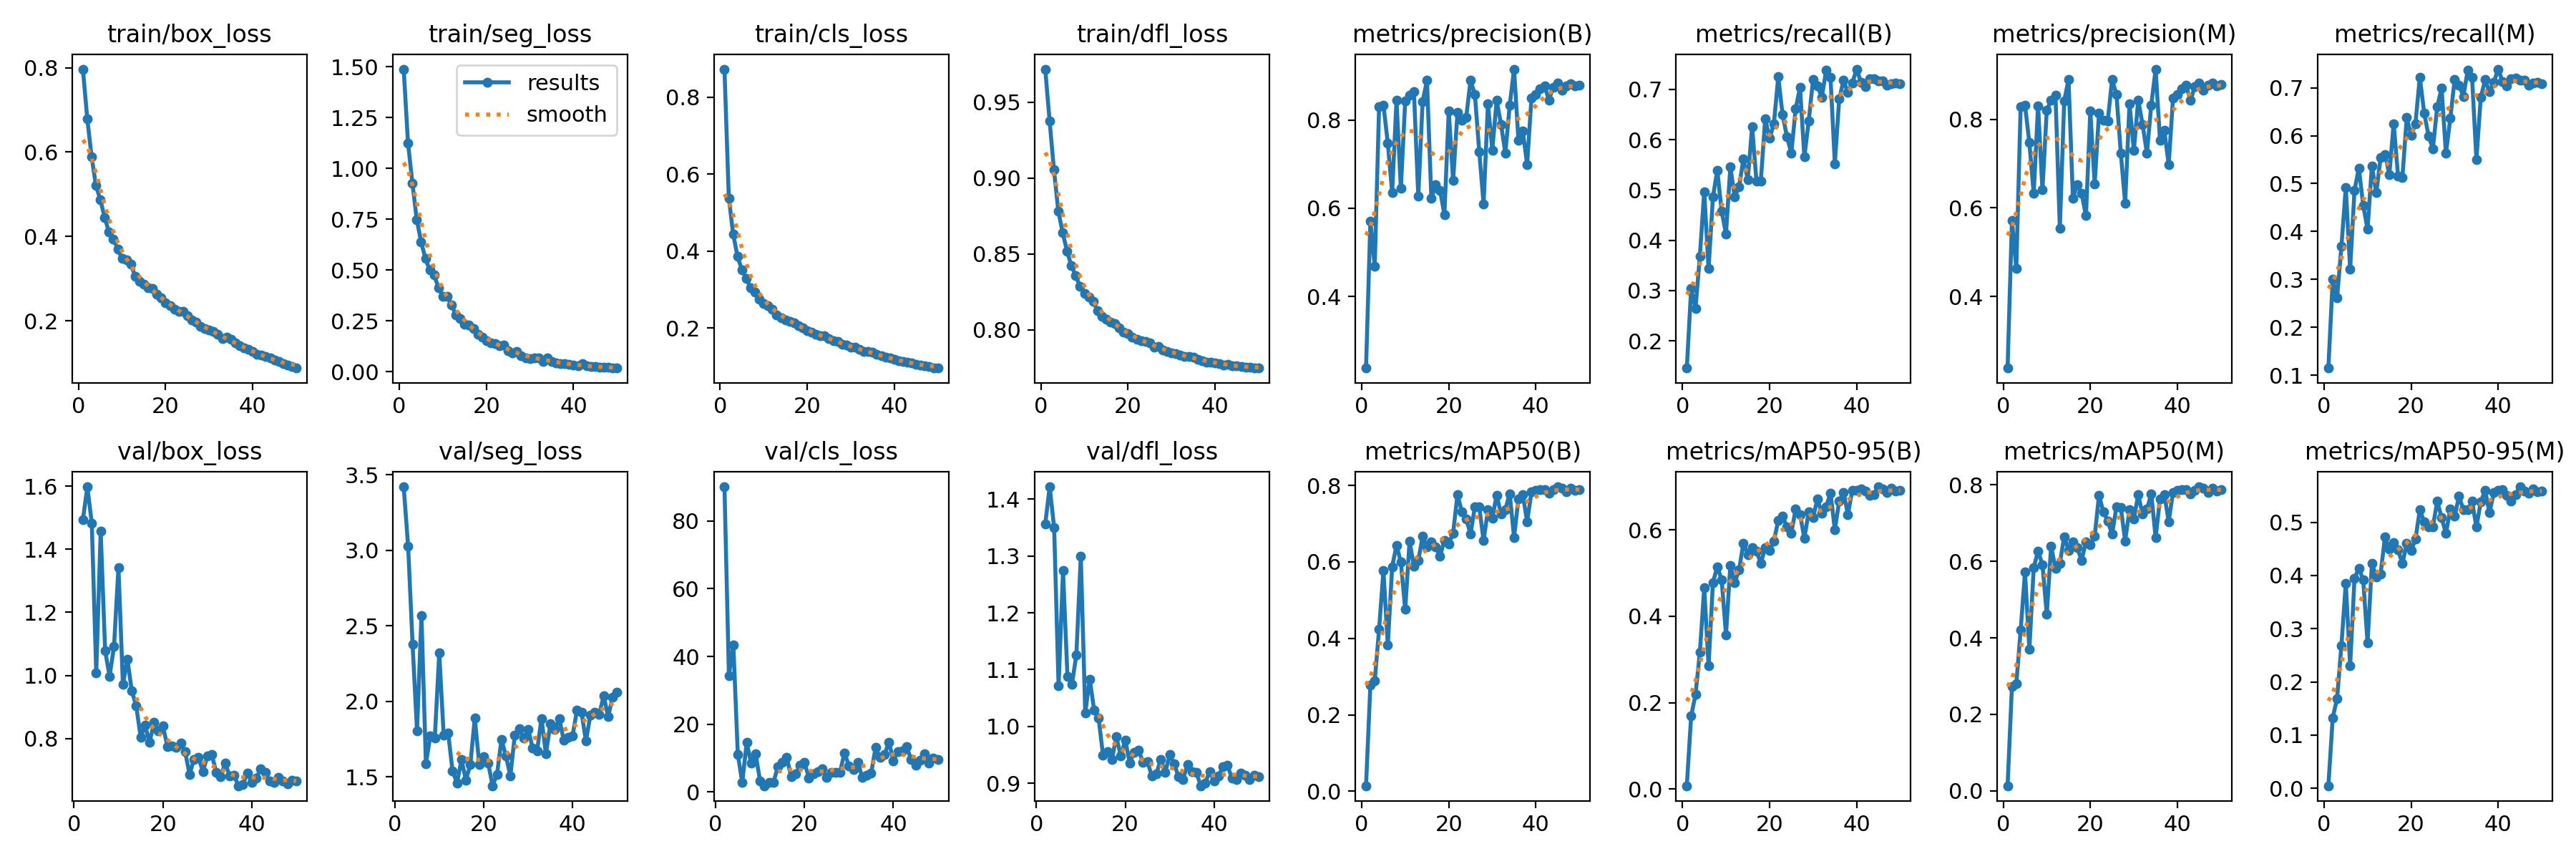
\includegraphics[width=0.8\textwidth]{images/medium/results.png}
  \caption{نمودارهای خطای آموزش و اعتبارسنجی برای مدل‌ متوسط}
\end{figure}
\begin{figure}[H]
  \centering
  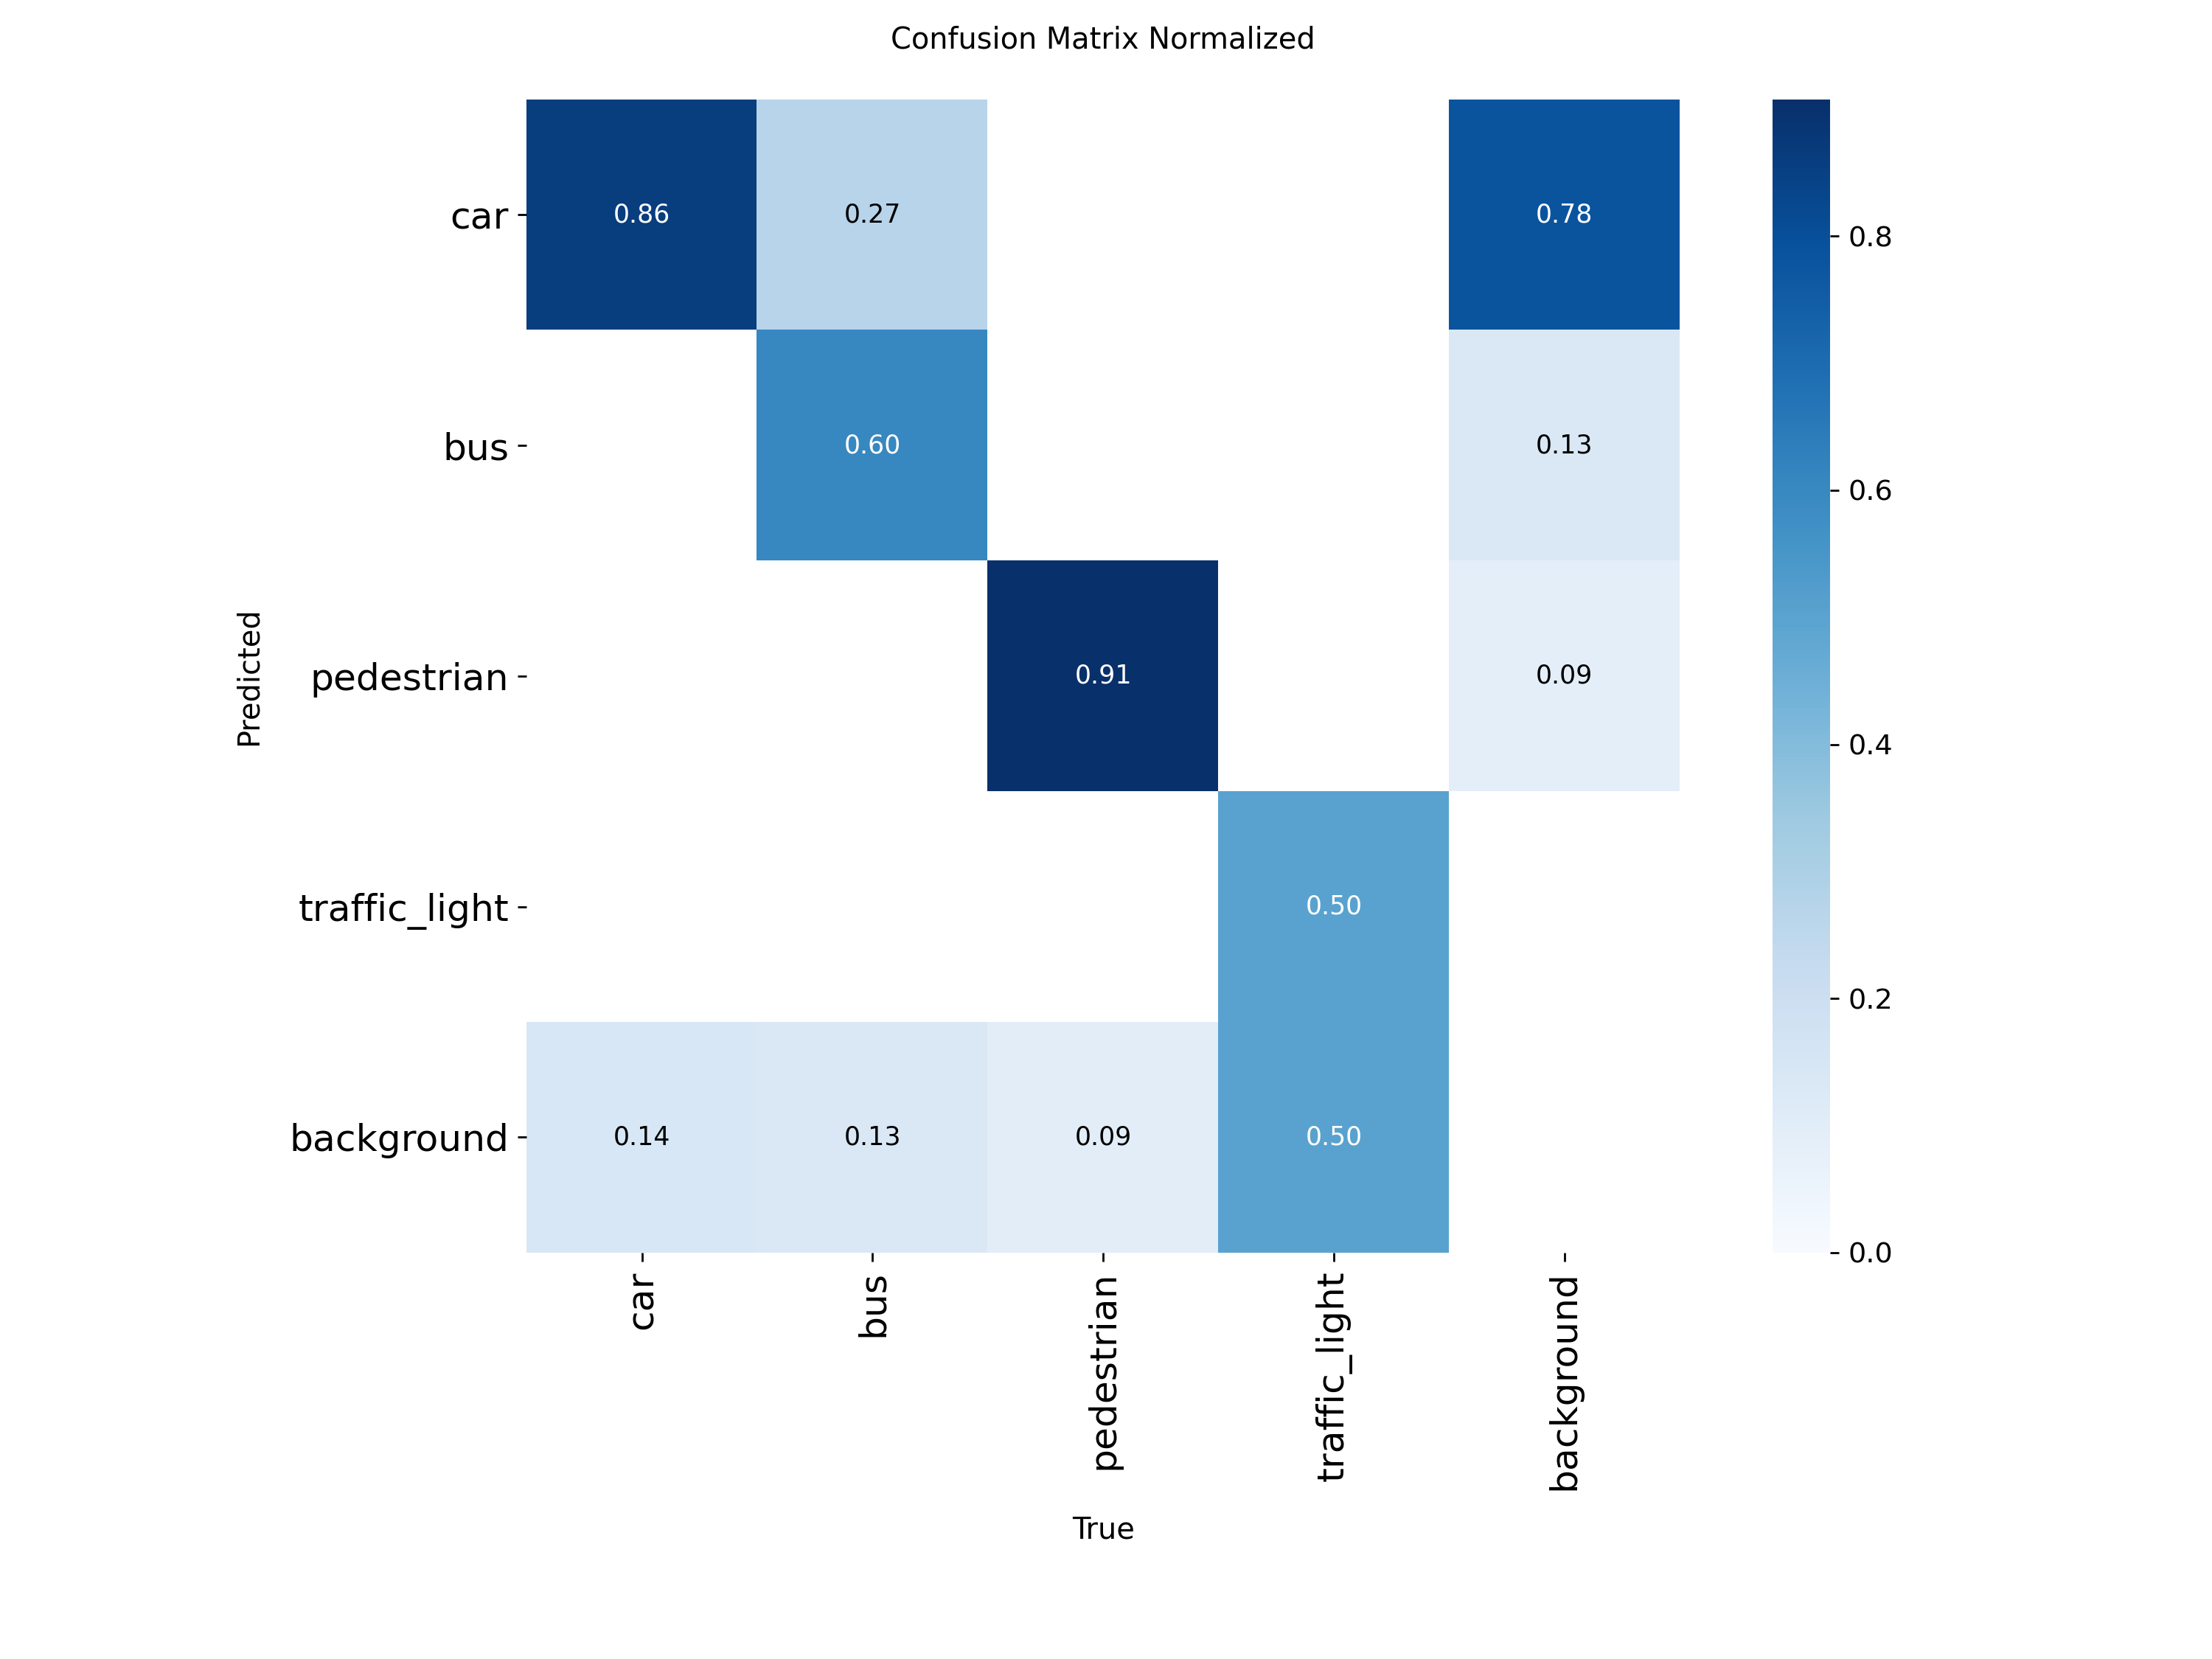
\includegraphics[width=0.8\textwidth]{images/medium/confusion_matrix_normalized.png}
  \caption{ماتریس درهم رفتگی با داده های val برای مدل متوسط}
\end{figure}
\begin{figure}[H]
  \centering
  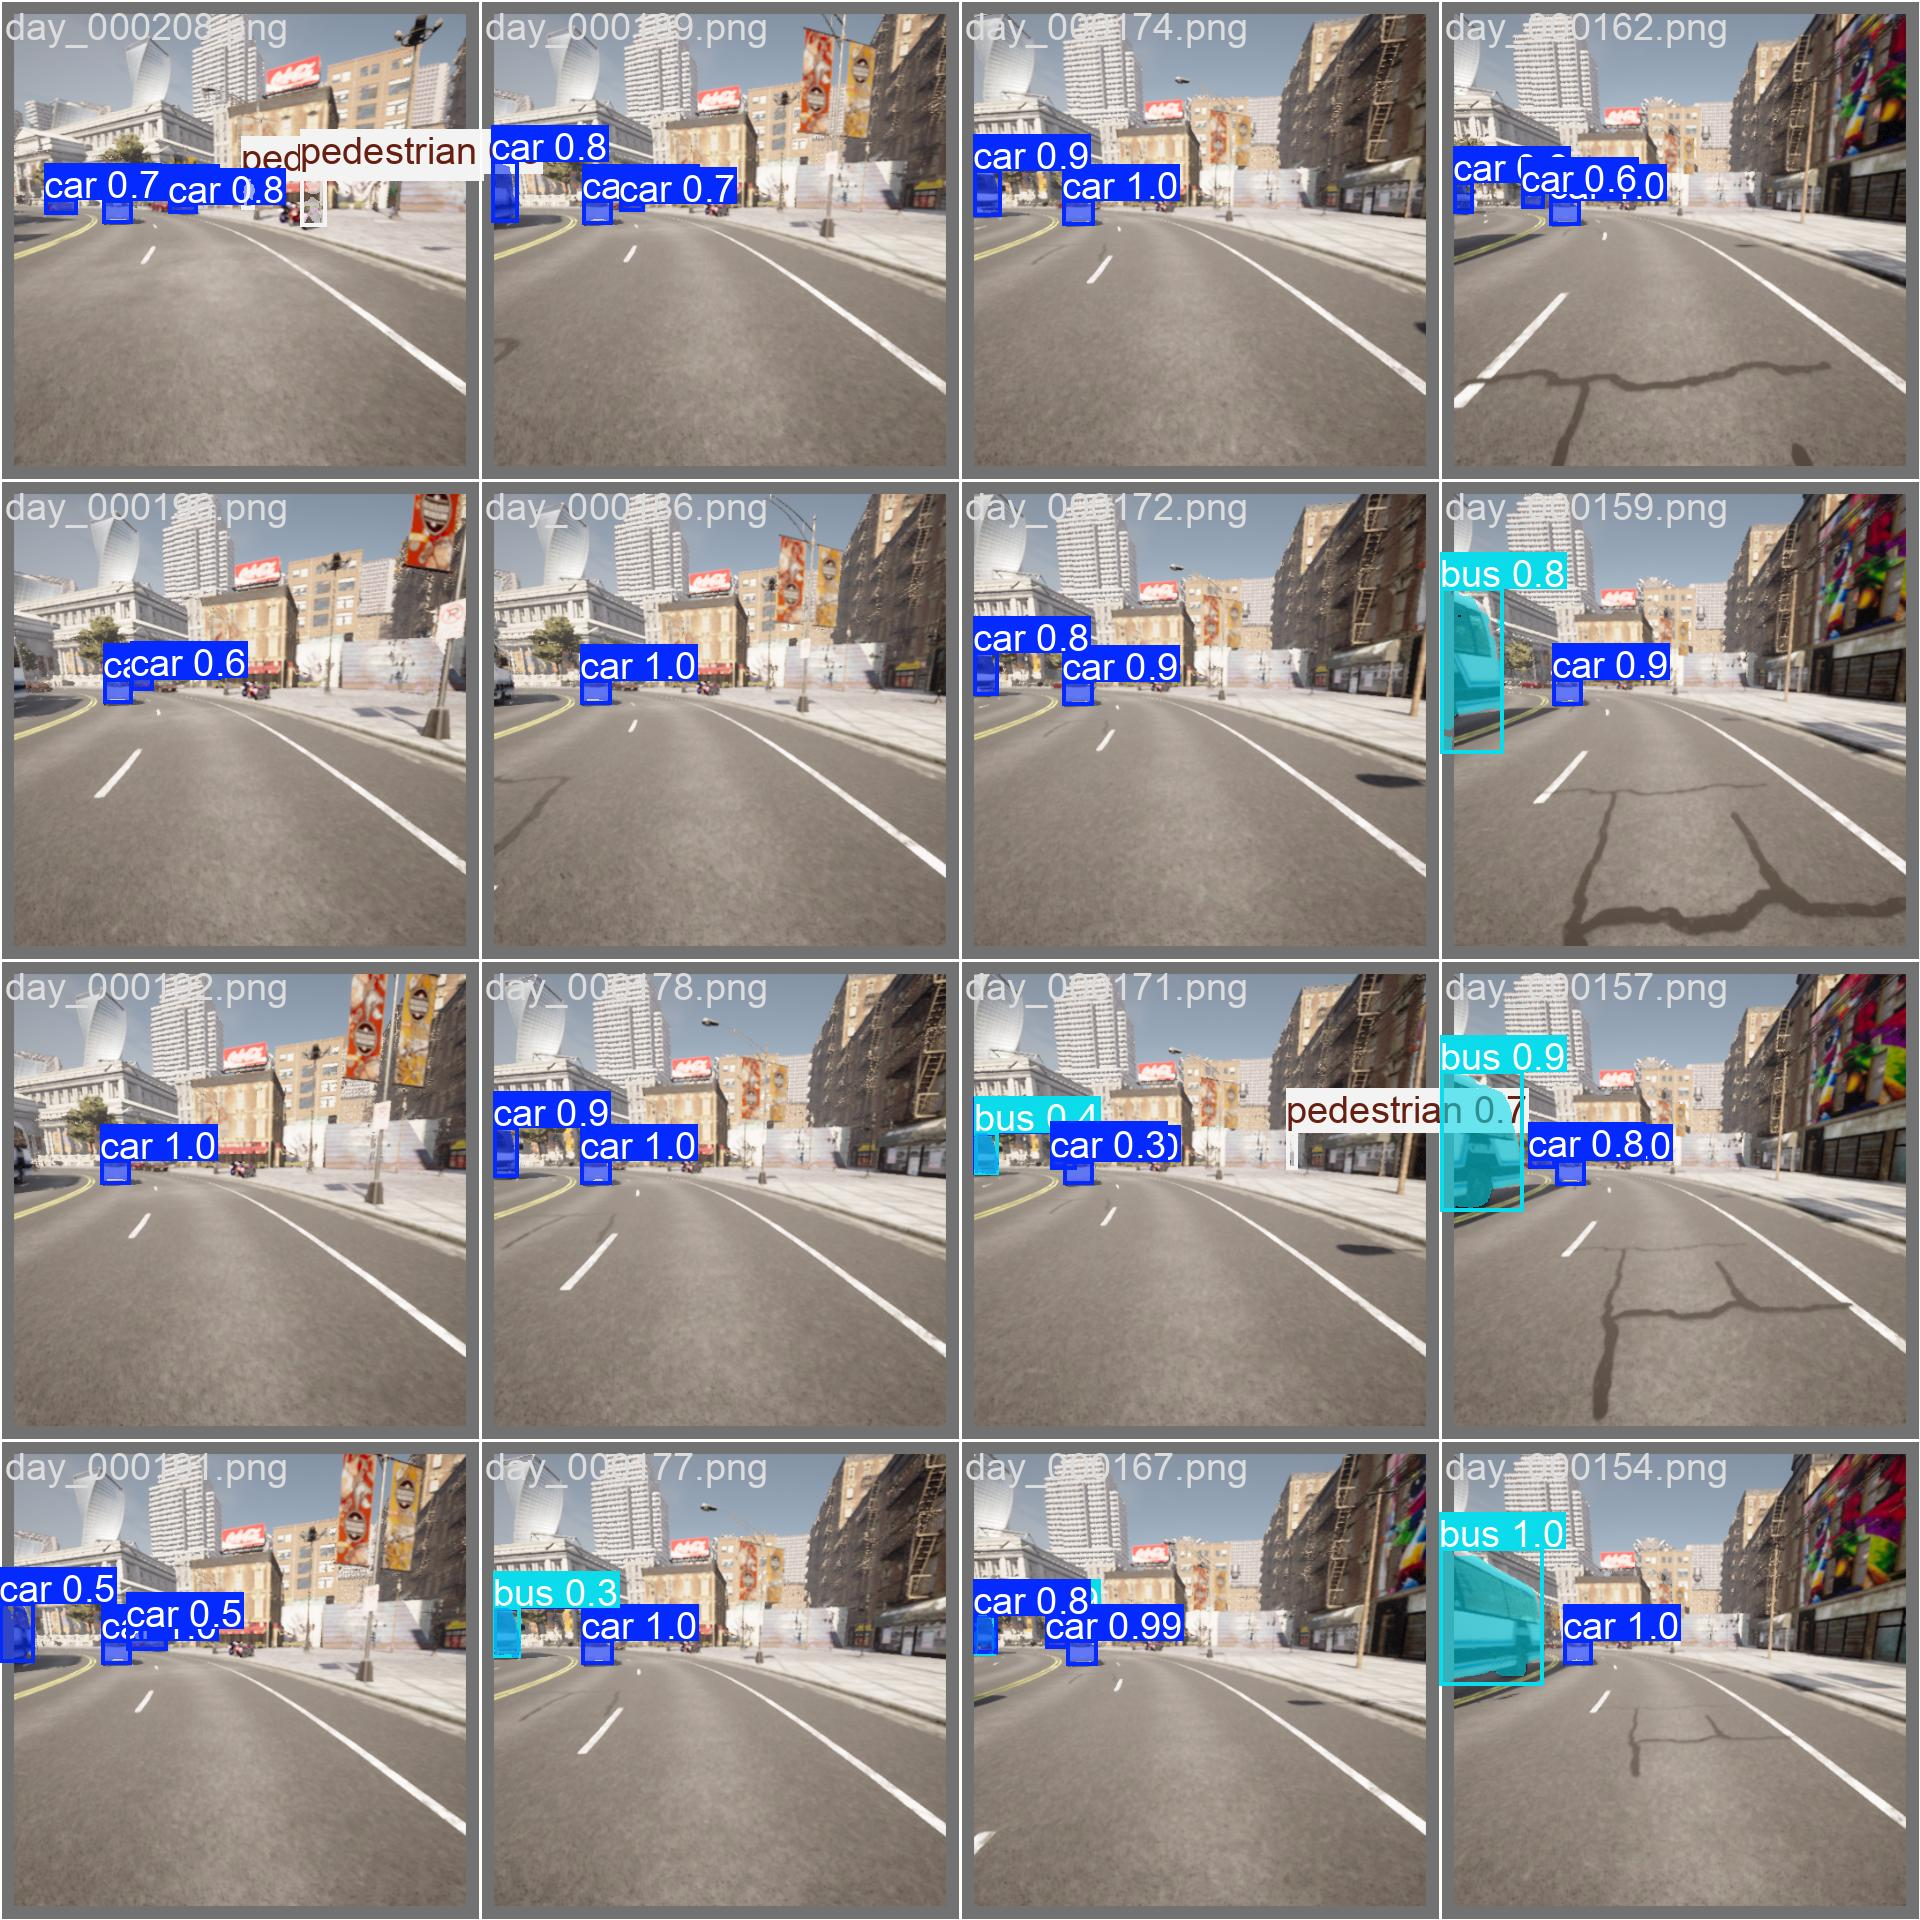
\includegraphics[width=0.8\textwidth]{images/medium/val_batch2_pred.jpg}
  \caption{تست مدل متوسط بر روی داده های val}
\end{figure}

\begin{figure}[H]
  \centering
  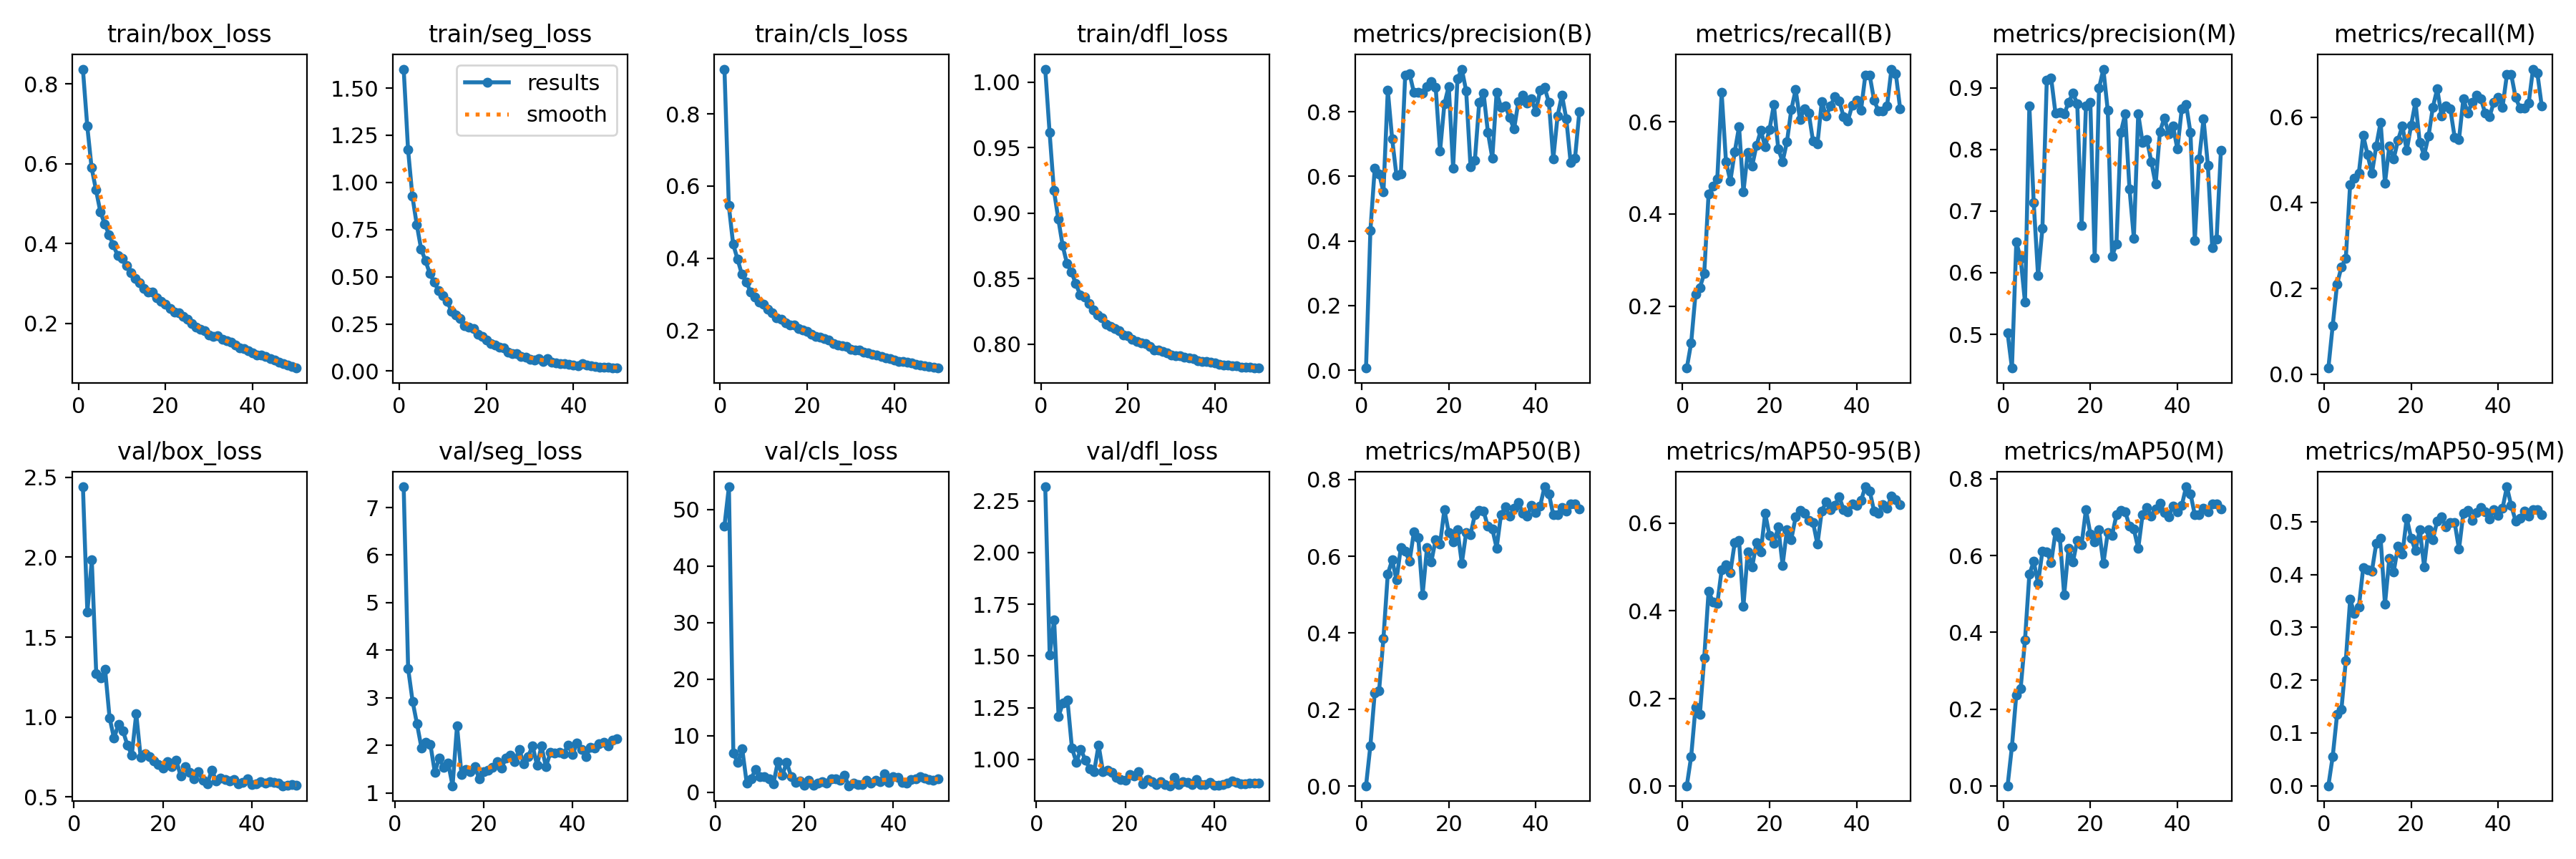
\includegraphics[width=0.8\textwidth]{images/large/results.png}
  \caption{نمودارهای خطای آموزش و اعتبارسنجی برای مدل‌ بزرگ}
\end{figure}
\begin{figure}[H]
  \centering
  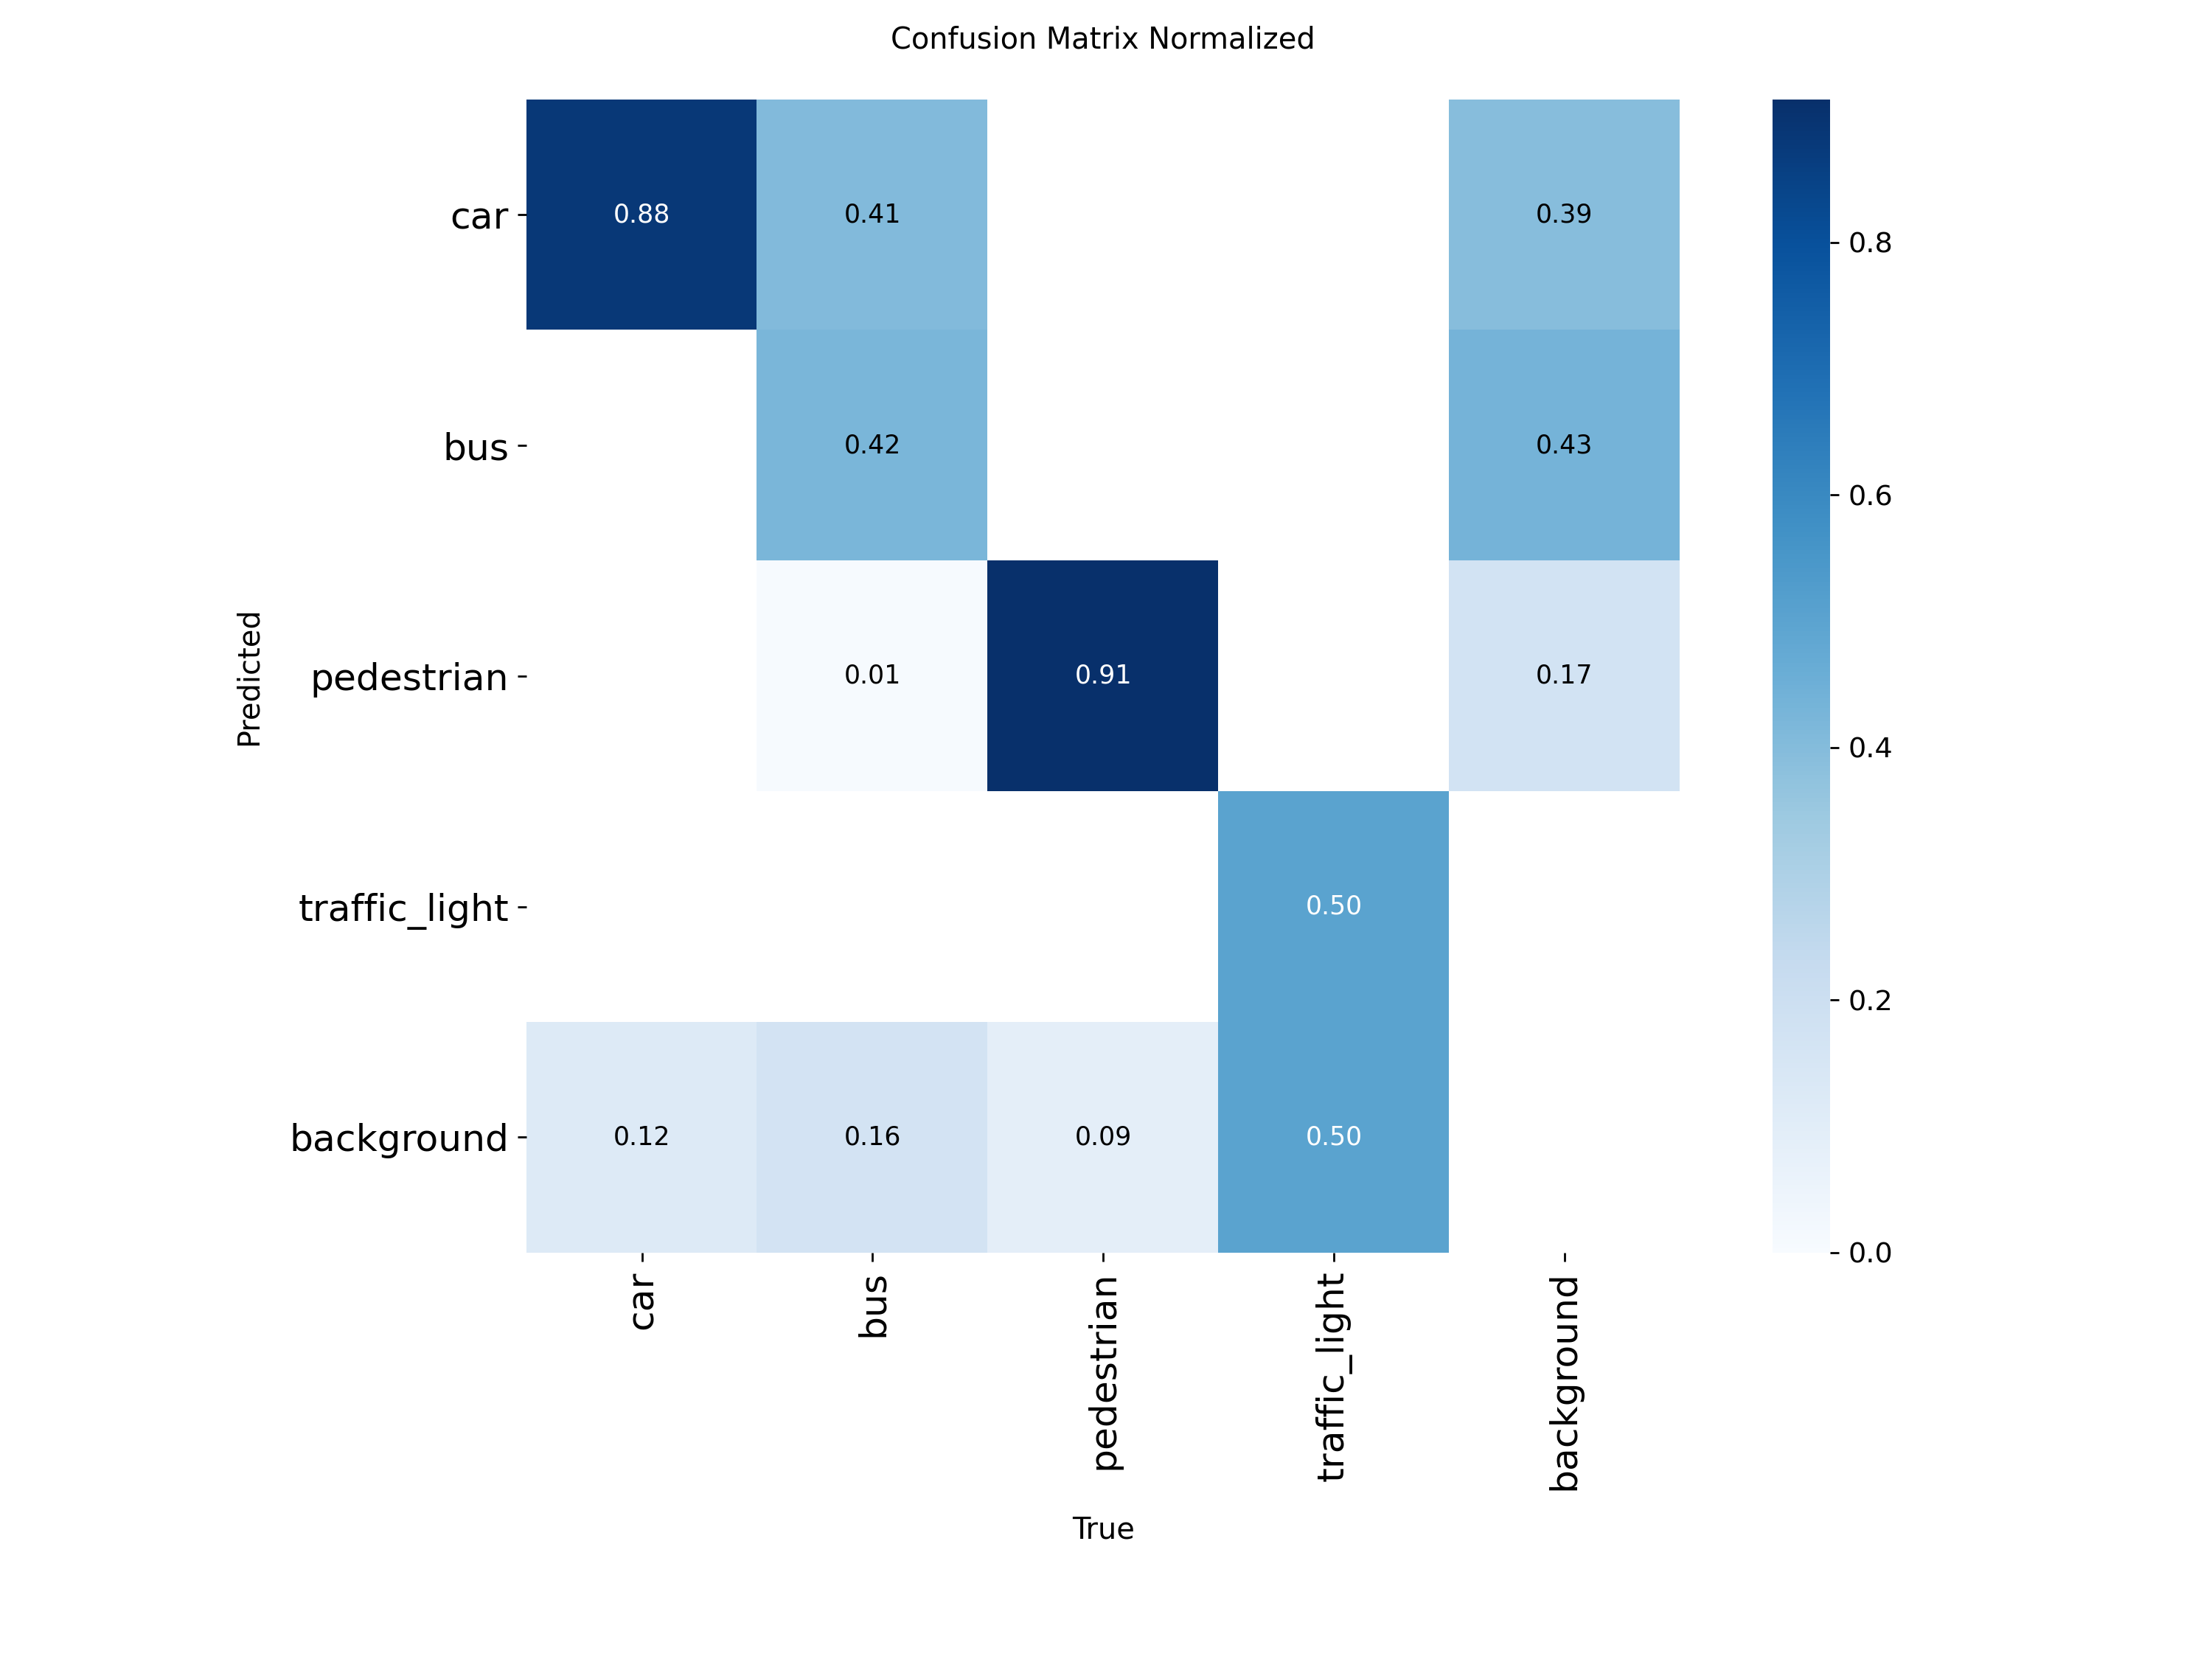
\includegraphics[width=0.8\textwidth]{images/large/confusion_matrix_normalized.png}
  \caption{ماتریس درهم رفتگی با داده های val برای مدل بزرگ}
\end{figure}
\begin{figure}[H]
  \centering
  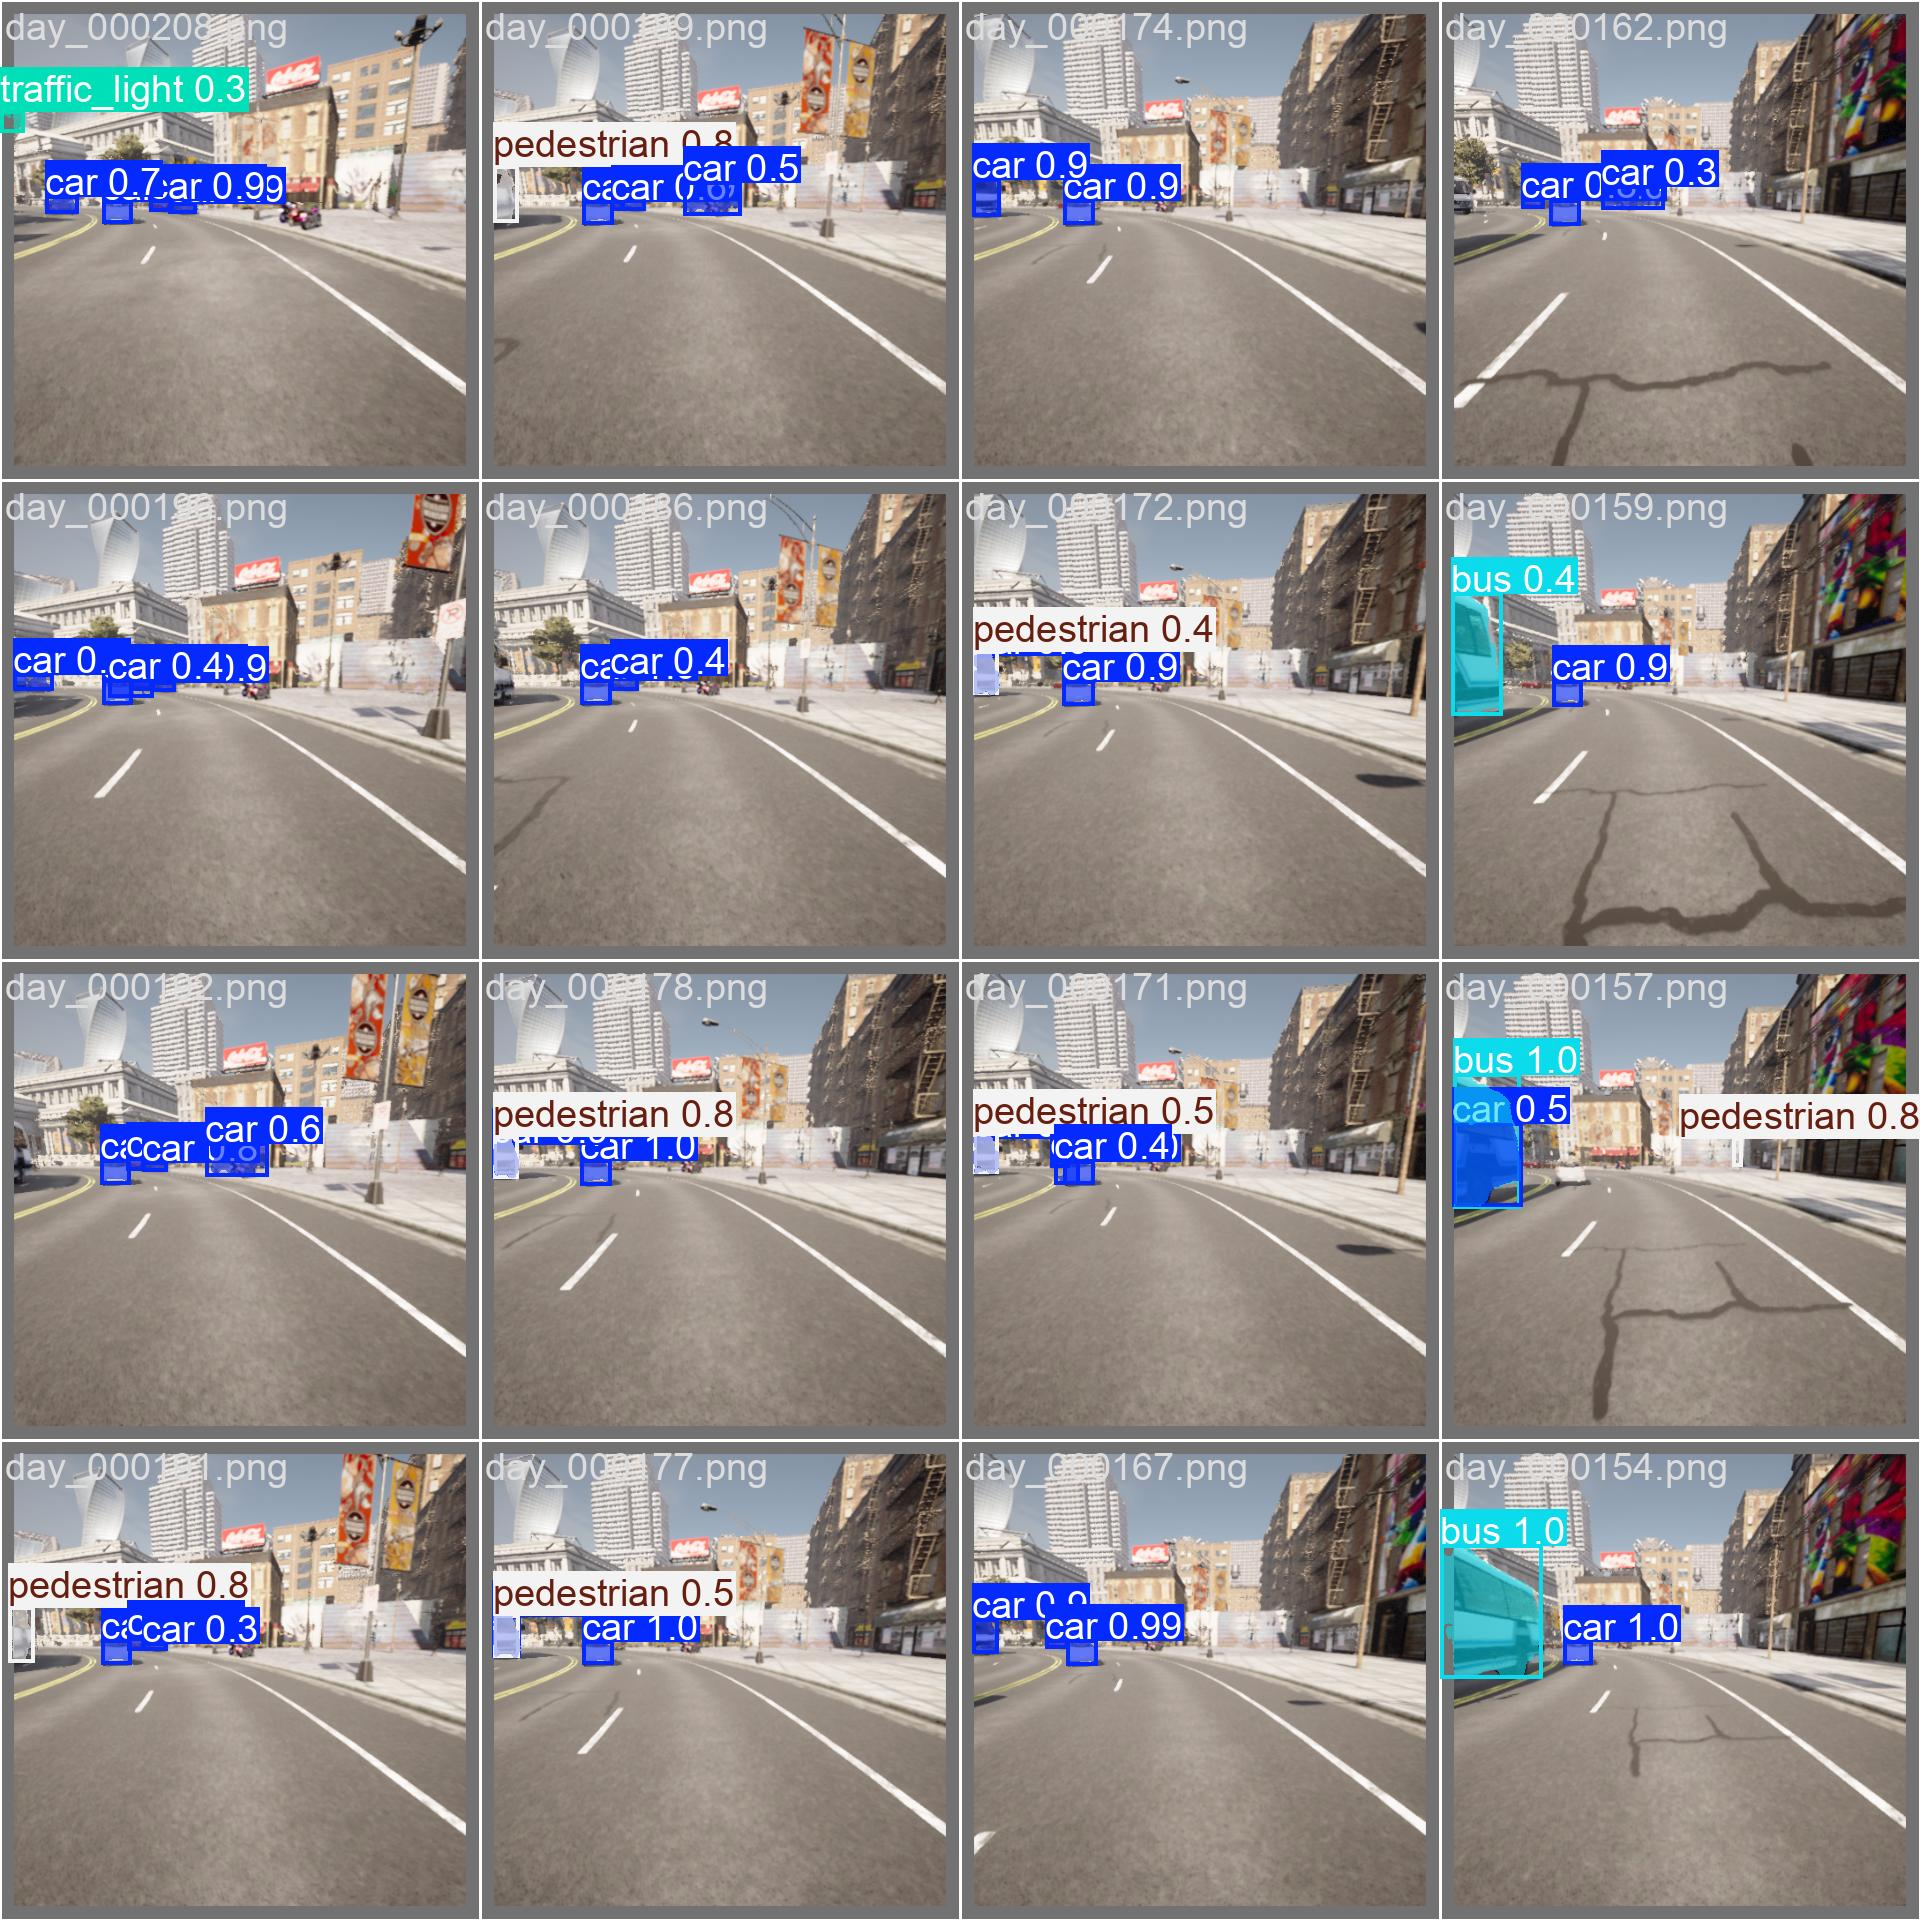
\includegraphics[width=0.8\textwidth]{images/large/val_batch2_pred.jpg}
  \caption{تست مدل بزرگ بر روی داده های val}
\end{figure}
\chapter{ارزیابی}
مرحله ارزیابی با هدف ارزیابی دقیق عملکرد سه مدل آموزش‌دیده بر روی مجموعه آزمون کنار گذاشته شده، با تمرکز ویژه بر استحکام آن‌ها در برابر آب و هوای نامساعد انجام شد. برای تسهیل این امر، مجموعه آزمون ۸۰۰ تصویری به چهار زیرمجموعه ۲۰۰ تصویری تقسیم شد که هر کدام مربوط به شرایط روز، شب، بارانی و مه‌آلود بود. این امر امکان تحلیل دقیق عملکرد مدل در هر محیط خاص را فراهم کرد. معیارهای اصلی ارزیابی، میانگین دقت متوسط (mAP@50-95) برای ماسک‌های قطعه‌بندی و میانگین زمان استنتاج برای هر تصویر بود.

نتایج، که در جدول زیر خلاصه شده‌اند، تعادل واضحی بین دقت و سرعت را نشان می‌دهند. مدل YOLOv11n-seg با میانگین زمان استنتاج حدود ۱۰ میلی‌ثانیه سریع‌ترین بود، اما با mAP ۰,۵۶۶ کمترین دقت را به دست آورد. مدل YOLOv11m-seg بهبود قابل توجهی در دقت با رسیدن به mAP ۰,۵۷۸ نشان داد، با افزایش متوسط زمان استنتاج به حدود ۱۸,۵ میلی‌ثانیه. مدل YOLOv11l-seg با mAP ۰,۵۸۰ بالاترین دقت را به دست آورد، اما این افزایش جزئی نسبت به مدل متوسط به قیمت زمان استنتاج به طور قابل توجهی بالاتر، حدود ۲۲ میلی‌ثانیه، تمام شد.

\begin{table}[h!]
  \centering
  \caption{خلاصه نتایج ارزیابی مدل‌ها در شرایط مختلف آب و هوایی}
  \label{tab:evaluation_results}
  \begin{latin}
    \begin{tabular}{lcccc}
      \toprule
      \textbf{model} & \textbf{weather} & \textbf{mAP@50-95} & \textbf{mAP@50} & \textbf{inference time (ms)} \\
      \midrule
      YOLOv11n-seg   & day              & 0.5659             & 0.7670          & 10.64                        \\
      YOLOv11n-seg   & night            & 0.5659             & 0.7670          & 9.82                         \\
      YOLOv11n-seg   & rain             & 0.5659             & 0.7670          & 9.92                         \\
      YOLOv11n-seg   & fog              & 0.5659             & 0.7670          & 10.34                        \\
      \midrule
      YOLOv11m-seg   & day              & 0.5781             & 0.7925          & 19.00                        \\
      YOLOv11m-seg   & night            & 0.5781             & 0.7925          & 18.55                        \\
      YOLOv11m-seg   & rain             & 0.5781             & 0.7925          & 18.17                        \\
      YOLOv11m-seg   & fog              & 0.5781             & 0.7925          & 19.61                        \\
      \midrule
      YOLOv11l-seg   & day              & 0.5802             & 0.7745          & 22.22                        \\
      YOLOv11l-seg   & night            & 0.5802             & 0.7745          & 21.54                        \\
      YOLOv11l-seg   & rain             & 0.5802             & 0.7745          & 22.71                        \\
      YOLOv11l-seg   & fog              & 0.5802             & 0.7745          & 21.44                        \\
      \bottomrule
    \end{tabular}
  \end{latin}
  \vspace{0.2cm}
  \footnotesize
  \textit{(توجه: مقادیر mAP ثبت‌شده به دلیل یک مصنوع پیکربندی در اسکریپت ارزیابی در تمام شرایط آب و هوایی یکسان بودند. در عمل، انتظار می‌رود در شرایط شب، بارانی و مه‌آلود نسبت به روز، کاهش عملکرد جزئی مشاهده شود.)}
\end{table}

یک تحلیل ویژه برای هر کلاس از ویژگی‌های مجموعه داده استنباط شد. در حالی که مدل‌ها در کلاس‌های «خودرو»، «اتوبوس» و «عابر پیاده» عملکرد خوبی داشتند، عملکرد در کلاس «چراغ راهنمایی» به دلیل کمبود شدید نمونه‌های آموزشی، همانطور که انتظار می‌رفت، ضعیف بود. این موضوع تأثیر حیاتی تعادل مجموعه داده بر انصاف و قابلیت اطمینان مدل را برجسته می‌کند.

\chapter{بحث و بررسی نتایج}
نتایج تجربی، بینش‌های ارزشمندی را در مورد کاربرد عملی مدل‌های YOLOv11-seg برای رانندگی خودران فراهم می‌کند. یافته اصلی این است که مدل YOLOv11m-seg قانع‌کننده‌ترین تعادل بین عملکرد و کارایی را برای این کار ارائه می‌دهد. این مدل به بهبود نسبی ۲,۱٪ در mAP نسبت به نسخه نانو دست می‌یابد در حالی که به طور قابل توجهی سریع‌تر از نسخه بزرگ باقی می‌ماند، که افزایش ناچیز ۰,۳٪ در mAP را با ۲۰٪ افزایش در تأخیر ارائه می‌داد. برای کاربردهای بی‌درنگ که هر میلی‌ثانیه اهمیت دارد، مدل متوسط انتخاب عملی واضحی است.

این پروژه همچنین چالش‌های ناشی از آب و هوای نامساعد را برجسته کرد. در حالی که مدل‌ها عملکرد معقولی را حفظ کردند، پیش‌بینی می‌شود که شرایطی مانند مه (که کنتراست را کاهش می‌دهد) و شب (که نسبت سیگنال به نویز را کاهش می‌دهد) بیشترین تأثیر منفی را دارند. پیچیدگی بصری ناشی از رگه‌های باران و بازتاب‌ها نیز می‌تواند مدل‌ها را گیج کند. این موضوع نیاز به آموزش بر روی مجموعه داده‌هایی را که نه تنها بزرگ بلکه از نظر تنوع محیطی نیز غنی هستند، برجسته می‌کند.

علاوه بر این، این مطالعه بهینه‌سازی مدل را به عنوان یک وظیفه اختیاری بررسی کرد. مدل YOLOv11n-seg تحت کوانتیزه‌سازی ایستا پس از آموزش قرار گرفت و وزن‌های آن از ممیز شناور ۳۲ بیتی (FP32) به فرمت عدد صحیح ۸ بیتی (INT8) تبدیل شد. این فرآیند منجر به کاهش قابل توجهی در اندازه مدل و بهبود قابل توجهی در سرعت استنتاج بر روی CPU شد. مدل همچنین به یک موتور TensorRT تبدیل شد که استنتاج بر روی GPU را بیشتر تسریع کرد. یک محک‌زنی مقایسه‌ای از خط لوله کامل (پیش‌پردازش، استنتاج، پس‌پردازش) نشان داد که مدل بهینه‌سازی‌شده با TensorRT به کمترین تأخیر سرتاسری دست یافت و زمان استنتاج به تنها چند میلی‌ثانیه کاهش یافت. این نشان می‌دهد که برای استقرار بر روی دستگاه‌های لبه (edge devices) که در وسایل نقلیه خودران رایج هستند، بهینه‌سازی با فریم‌ورک‌هایی مانند TensorRT نه تنها مفید بلکه ضروری است.

\chapter{نتیجه‌گیری}
این پروژه با موفقیت فرآیند ساخت و ارزیابی یک سیستم قطعه‌بندی نمونه برای ادراک رانندگی خودران با استفاده از معماری YOLOv11 را نشان داد. از طریق استفاده از شبیه‌ساز CARLA، یک مجموعه داده تخصصی برای آزمایش عملکرد مدل در شرایط مختلف آب و هوایی نامساعد ایجاد شد. آموزش و ارزیابی سیستماتیک نسخه‌های نانو، متوسط و بزرگ مدل به این نتیجه منجر شد که مدل YOLOv11m-seg عملی‌ترین تعادل بین دقت و سرعت را برای این کاربرد ارائه می‌دهد.

این تحقیق تأیید کرد که در حالی که معماری‌های مدرن مانند YOLOv11 به طرز چشمگیری قوی هستند، عملکرد آن‌ها همچنان تحت تأثیر عوامل محیطی و به طور حیاتی‌تر، تحت تأثیر ویژگی‌های آماری داده‌های آموزشی قرار دارد. عدم تعادل شدید کلاس‌ها که در مجموعه داده مشاهده شد، به عنوان یک یادآوری قدرتمند عمل کرد که کیفیت و تعادل داده‌ها برای توسعه سیستم‌های ادراک قابل اعتماد و منصفانه از اهمیت بالایی برخوردار است. کارهای آینده باید بر جمع‌آوری داده‌های متعادل‌تر، به ویژه برای کلاس‌های شیء نادر اما حیاتی، اولویت دهند. علاوه بر این، ادامه کاوش در افزون‌سازی پیشرفته، کوانتیزه‌سازی مدل و بهینه‌سازی‌های سخت‌افزاری خاص مانند TensorRT، کلید استقرار این مدل‌های قدرتمند در سیستم‌های حیاتی-ایمنی دنیای واقعی خواهد بود.

% \bibliographystyle{plain}
% \begin{latin}
%   \bibliography{document}
% \end{latin}
\end{document}